\chapter[Discretization and Primitivity of the Neutron Transport Criticality\\ Eigenvalue Problems][Discretization and Primitivity]{Discretization and Primitivity of the Neutron Transport Criticality Eigenvalue Problems}
%\chaptermark{Discretization and Primitivity of the Neutron Transport Criticality Eigenvalue Problems}
\label{Discrete}

In this section we describe the discretization of the neutron transport criticality eigenvalue equations for three-dimensional Cartesian geometry. The discretization follows a similar approach to that of Brown \cite{brown_linear_1995} \cite{brown_POI_2008} \cite{brown_POI_2012}. First, we derive semi-discretized forms of the eigenvalue equations by applying the \textit{multigroup}-in-energy approximation and a spherical harmonics expansion for the scattering integral. We then discretize the spatial and angular variables using step differencing and the discrete ordinates approach. Finally, we write down the discretized matrix forms of the criticality eigenvalue equations for three-dimensional Cartesian geometry. For the one-dimensional slab geometry discretized alpha-eigenvalue problem, we prove that the discretized transport equation matrix is primitive. A similar result can be shown for the two-dimensional and three-dimensional Cartesian discretized eigenvalue equations.

We begin with the linear alpha-eigenvalue neutron transport equation in a three-dimen\-sional box geometry. For a description of the discretization process for the one-dimensional slab neutron transport eigenvalue equations see Appendix~\ref{Discrete1D}. The spatial domain is the box $\mathcal{D} \equiv \{\vec{r} = (x, y, z) \, \vert \, a_{x} \leq x \leq b_{x}, a_{y} \leq y \leq b_{y}, \text{ and } a_{z} \leq z \leq b_{z} \},$ the direction variable is $\hat{\Omega} \in \mathcal{S}^{2}$, the unit sphere in $\mathbb{R}^{3}$, the energy variable is $E \in (0, \infty)$, and the equation for the angular flux $\psi(\vec{r}, \hat{\Omega}, E)$ is given by

\begin{multline}
	\bigg [ \frac{\alpha}{v(E)} + \hat{\Omega} \cdot \nabla + \sigma(\vec{r},E) \bigg ] \psi(\vec{r},\hat{\Omega},E) \\ = \int_{0}^{\infty} \diff E' \, \int_{4\pi} \diff \hat{\Omega}' \, \sigma_{s}(\vec{r},E'\rightarrow E,\hat{\Omega}' \cdot \hat{\Omega}) \psi(\vec{r},\hat{\Omega}',E') \\ + \int_{0}^{\infty} \diff E' \, \nu(E') \chi(E'\rightarrow E) \sigma_{f}(\vec{r},E') \int_{4\pi} \diff \hat{\Omega}' \, \psi(\vec{r},\hat{\Omega}',E'), 
	\label{eq:Alpha3DNeutronTransport}
\end{multline}
where
\begin{equation}
	\nabla \psi \equiv \bigg (\frac{\partial \psi}{\partial x}, \frac{\partial \psi}{\partial y}, \frac{\partial \psi}{\partial z} \bigg ),
\end{equation}
and
\begin{equation}
	 \int_{4\pi} \diff \hat{\Omega} = 1.
\end{equation}
In the discretization of Eq.~\ref{eq:Alpha3DNeutronTransport} it is assumed that $\chi(E' \rightarrow E)$ is not a function of the incident neutron energy $E'$. Therefore, we have 

\begin{equation}
\chi(E' \rightarrow E) = \chi(E).
\end{equation}

Boundary conditions must be specified to make Eq.~\ref{eq:Alpha3DNeutronTransport} well-posed. Various boundary conditions can be specified such as a reflecting condition on a face or a Dirichlet condition where an incident flux is specified on a face. We consider vacuum boundary conditions in this dissertation, a special case of the Dirichlet boundary condition where no incident flux is imposed:

\begin{equation}
	\psi(\vec{r},\hat{\Omega},E) = 0 \text{ for all } \vec{r} \in \partial \mathcal{D} \text{ and } \hat{\Omega} \in \mathcal{S}^{2} \text{ with } \vec{n}(\vec{r}) \cdot \hat{\Omega} < 0,
\end{equation}
where $\vec{n}(\vec{r})$ is the outward pointing unit normal at $\vec{r} \in \partial \mathcal{D}$.

\section{Discretization of the Alpha-Eigenvalue and $k$-Effective Eigenvalue Equations}

In this section, we discuss the discretization of the alpha- and $k$-effective eigenvalue neutron transport equations. We begin by approximating the energy dependence of the neutron transport equations using the multigroup-in-energy approximation. We then discretize the angular flux and scattering cross sections using a surface harmonics expansion. Finally, the spatial and angular dependences of the eigenvalue equations are then approximated using step differencing in space and the discrete ordinates approach in angle.

\subsection{The Multigroup-in-Energy Discretization and Surface Harmonics Expansion of the Angular Flux}

\subsubsection{The Multigroup-in-Energy Approximation}

We begin by discretizing Eq.~\ref{eq:Alpha3DNeutronTransport} in energy using the \textit{multigroup} approximation \cite{duderstadt_nuclear_1976}. We restrict the energy $E$ to a finite interval and partition the interval into groups:
\begin{equation*}
	E_{max} = E_{0} > E_{1} > \dots > E_{G} = E_{min}.
\end{equation*}
The eigenvalue equation is then integrated over each group $E_{g} < E < E_{g-1}$ and the cross sections are approximated by a flat-flux weighting over each energy group to yield the following semi-discretization of Eq.~\ref{eq:Alpha3DNeutronTransport}:
\begin{multline}
	\bigg [ \frac{\alpha}{v_{g}} + \hat{\Omega} \cdot \nabla + \sigma_{g}(\vec{r}) \bigg ] \psi_{g}(\vec{r},\hat{\Omega}) = \sum_{g'=1}^{G} \int_{4\pi} \diff \hat{\Omega'} \, \sigma_{s,g,g'}(\vec{r},\hat{\Omega}' \cdot \hat{\Omega}) \psi_{g'}(\vec{r},\hat{\Omega}') \\ + \chi_{g} \sum_{g'=1}^{G} \, \nu\sigma_{f,g'}(\vec{r}) \int_{4\pi} \diff \hat{\Omega}' \, \psi_{g'}(\vec{r},\hat{\Omega}'), 
	\label{eq:Alpha3DMG}
\end{multline}
for $g = 1, \dots, G$, where
\begin{equation}
	\psi_{g}(\vec{r},\hat{\Omega}) \equiv \int_{g} \diff E \, \psi(\vec{r},\hat{\Omega},E),
\end{equation}
\begin{equation}
	 \sigma_{g}(\vec{r}) \equiv \frac{1}{\Delta E_{g}} \int_{g} \diff E \, \sigma(\vec{r},E),
\end{equation}
\begin{equation}
	 \sigma_{s,g,g'}(\vec{r},\hat{\Omega}' \cdot \hat{\Omega}) \equiv \frac{1}{\Delta E_{g'}} \int_{g} \int_{g'} \diff E' \diff E \, \sigma_{s}(\vec{r},E'\rightarrow E,\hat{\Omega}' \cdot \hat{\Omega}),
\end{equation}
\begin{equation}
	\nu\sigma_{f,g}(\vec{r}) \equiv \frac{1}{\Delta E_{g}} \int_{g} \diff E \, \nu(E) \sigma_{f}(E),
\end{equation}
\begin{equation}
	\chi_{g} \equiv \int_{g} \diff E \, \chi(E),
\end{equation}
with
\begin{equation}
	\int_{g} \diff E \, = \int_{E_{g}}^{E_{g-1}} \diff E.
\end{equation}
We note that 
\begin{equation}
	\sum_{g=1}^{G} \chi_{g} = 1
\end{equation}
in the multigroup formulation since
\begin{equation}
	\int_{0}^{\infty} \diff E \, \chi(E) = 1.
\end{equation}

\subsubsection{The Surface Harmonics Expansion of the Angular Flux}

For each flux $\psi_{g}(\vec{r},\hat{\Omega})$, the flux is expanded in surface harmonics according to
\begin{equation}
	\psi_{g}(\vec{r},\hat{\Omega}) = \sum_{n=0}^{\infty} \sum_{m=-n}^{n} \phi_{g,n,m}(\vec{r}) Y_{n}^{m}(\hat{\Omega}),
\end{equation}
where $Y_{n}^{m}(\hat{\Omega})$ is a surface harmonic defined as
\begin{equation}
	Y_{n}^{m}(\hat{\Omega}) = a_{n}^{m} P_{n}^{\abs{m}}(\xi) \tau_{m}(\varphi),
\end{equation}
\begin{equation}
\hat{\Omega} = (\sin \theta \cos \varphi, \sin \theta \sin \varphi, \cos \theta),
\end{equation}
\begin{equation}
	\tau_{m}(\varphi) = \begin{cases}
					\cos m\varphi, \quad \text{if } m \geq 0, \\
					\sin \abs{m} \varphi \quad \text{if } m < 0,
				      \end{cases}
\end{equation}
and $P_{n}^{\abs{m}}$ is an \textit{associated Legendre polynomial} \cite{duderstadt_nuclear_1976}. The constants $a_{n}^{m}$ are defined by
\begin{equation}
	a_{n}^{m} = \bigg [ \frac{2(2n+1)(n-\abs{m})!}{(1+\delta_{m0})(n + \abs{m})!} \bigg ]^{1/2}.
\end{equation}
where $\delta_{n,n'}$ is the \textit{Kronecker delta}. The $(n,m)^{\text{th}}$ moment of $\psi(\vec{r}, \hat{\Omega})$, $\phi_{n,m}$ is given by
\begin{equation}
	\phi_{n,m}(\vec{r}) = \int_{4\pi} \diff \hat{\Omega} \, \psi(\vec{r},\hat{\Omega}) Y_{n}^{m}(\hat{\Omega}).
\end{equation}

From the properties of the surface harmonics, we have
\begin{equation}
	\int_{4\pi} \diff \hat{\Omega} \, Y_{n}^{m}(\hat{\Omega}) Y_{n'}^{m'}(\hat{\Omega}) = \delta_{n,n'} \delta_{m,m'}, \text{ for all } n, n' = 0, 1, \dots, \abs{m} \leq \abs{n}, \abs{m'} \leq \abs{n'}.
\end{equation}
The scattering integral can be then be written in the form
\begin{equation}
	\int_{4\pi} \diff \hat{\Omega}' \, \sigma_{s,g,g'}(\vec{r},\hat{\Omega}' \cdot \hat{\Omega}) \psi_{g'}(\vec{r},\hat{\Omega}') = \sum_{n=0}^{\infty} \sigma_{s,g,g',n}(\vec{r}) \sum_{m=-n}^{n} \phi_{g',n,m}(\vec{r})Y_{n}^{m}(\hat{\Omega}),
	\label{eq:ScattInt}
\end{equation}
where
\begin{equation}
	\sigma_{s,g,g',n}(\vec{r}) \equiv \frac{1}{2} \int_{-1}^{1} \diff \mu_{0} \, \sigma_{s,g,g'}(\vec{r},\mu_{0}) P_{n}(\mu_{0}),
\end{equation}
and $\mu_{0}$ is the cosine of the scattering angle. The infinite series in Eq.~\ref{eq:ScattInt} is truncated to a finite number of terms $N_{s}$, where $N_{s}$ is the maximum value for $n$. If fission is not assumed to be isotropic the fission integral can be written similarly with the infinite series truncated after $N_{f}$ terms. If fission is isotropic, the expansion simplifies to only a function of the neutron scalar flux. The multigroup equations can then be written as
\begin{multline}
	\bigg [ \frac{\alpha}{v_{g}} + \hat{\Omega} \cdot \nabla + \sigma_{g}(\vec{r}) \bigg ] \psi_{g}(\vec{r},\hat{\Omega}) = \sum_{g'=1}^{G} \sum_{n=0}^{N_{s}} \sigma_{s,g,g',n}(\vec{r}) \sum_{m=-n}^{n} \phi_{g',n,m}(\vec{r}) Y_{n}^{m}(\hat{\Omega}) \\ + \chi_{g} \sum_{g'=1}^{G} \sum_{n=0}^{N_{f}} \nu\sigma_{f,g',n}(\vec{r}) \sum_{m=-n}^{n} \phi_{g',n,m}(\vec{r}) Y_{n}^{m}(\hat{\Omega}), 
	\label{eq:Alpha3DMGSPH}
\end{multline}
for $g = 1, \dots, G$.

\subsection{Step Differencing in Space and Discrete Ordinates in Angle}

\subsubsection{Step Differencing}

We continue the discretization of Eq.~\ref{eq:Alpha3DMGSPH} by using a Step finite differencing method \cite{lewis_computational_1984} for the spatial variable $\vec{r}$. We start with the three-dimensional mono-energetic alpha-eigenvalue equation for group $g$ with scattering and fission source $f$:

\begin{equation}
\begin{cases}
	\frac{\alpha}{v} \psi + \hat{\Omega} \cdot \nabla \psi + \sigma \psi = f \text{ in } \mathcal{D} \\
	\psi(\vec{r}) = 0 \text{ for all } \vec{r} \in \partial \mathcal{D} \text { with } \vec{n}(\vec{r}) \cdot \hat{\Omega} < 0.
\end{cases}
\label{eq:ContG}
\end{equation}
We discretize the domain $\mathcal{D}$ into zones and define
\begin{equation}
	\Delta x_{i} = x_{i} - x_{i-1}, \text{ for } i = 1, \dots, M,
\end{equation}
\begin{equation}
	\Delta y_{j} = y_{j} - y_{j-1}, \text{ for } j = 1, \dots, J,
\end{equation}
\begin{equation}
	\Delta z_{k} = z_{k} - z_{k-1}, \text{ for } k = 1, \dots, K.
\end{equation}
We define the nodes $r_{ijk} = (x_{i}, y_{j}, z_{k})$ and the zone volume $\Delta r_{ijk} = \Delta x_{i} \Delta y_{j} \Delta z_{k}$. The function values at the set of nodes, $\{r_{ijk}\}$ are called \textit{nodal values}. We assume that $\sigma$ and $f$ have constant values, denoted as $\sigma_{ijk}$ and $f_{ijk}$ respectively, on each \textit{zone} defined as
\begin{equation}
	\mathcal{Z}_{ijk} \equiv \{ r \vert x_{i-1} < x < x_{i}, y_{j-1} < y < y_{j}, z_{k-1} < z < z_{k} \}.
\end{equation}
We define $\psi_{ijk}$ to denote the approximation to $\psi(r_{ijk})$, the true solution at the point $r_{ijk}$. 

For a direction in the positive orthant, $\hat{\Omega} = (\mu, \eta, \xi) > 0$, the Step differencing equation for the zone $\mathcal{Z}_{ijk}$ is
\begin{equation}
	\frac{\alpha}{v} \psi_{ijk} + \mu \frac{\psi_{ijk} - \psi_{i-1,jk}}{\Delta x_{i}} + \eta \frac{\psi_{ijk} - \psi_{i,j-1,k}}{\Delta y_{j}} + \xi \frac{\psi_{ijk} - \psi_{ij,k-1}}{\Delta z_{k}} + \sigma_{ijk} \psi_{ijk} = f_{ijk}.
	\label{eq:Step3D}
\end{equation}
For Eq.~\ref{eq:Step3D}, we have $(M+1)(J+1)(K+1)$ unknowns $\psi_{ijk}$. There are $MJK$ zonal equations with $JM + JK + M + J + K + 1$ boundary equations.

To write the discretized system in matrix form, we define the discrete angular flux vector
\begin{equation}
\Psi \in \mathbb{R}^{(M+1)(J+1)(K+1)},
\end{equation}
defined for all nodes ordered by $i$ first, then $j$, and finally $k$. We define the diagonal matrices
\begin{equation}
	\Delta x \equiv \text{diag}(\Delta x_{1}, \dots, \Delta x_{M}),
\end{equation}
\begin{equation}
	\Delta y \equiv \text{diag}(\Delta y_{1}, \dots, \Delta y_{J}),
\end{equation}
\begin{equation}
	\Delta z \equiv \text{diag}(\Delta z_{1}, \dots, \Delta z_{K}),
\end{equation}
and the matrices expressing the discretized spatial derivatives 
\begin{equation}
	D_{M} \in \mathbb{R}^{M \times (M+1)} \equiv \begin{pmatrix}
				-1 & 1 & &  \\
				& \ddots & \ddots  & \\
				& & -1 & 1
		             \end{pmatrix},
	S_{M,+} \in \mathbb{R}^{M \times (M+1)} \equiv \begin{pmatrix}
				0 & 1 & &  \\
				& \ddots & \ddots  & \\
				& & 0 & 1
				\end{pmatrix},
\end{equation}
\begin{equation}
	D_{J} \in \mathbb{R}^{J \times (J+1)} \equiv \begin{pmatrix}
				-1 & 1 & &  \\
				& \ddots & \ddots  & \\
				& & -1 & 1
		             \end{pmatrix},
	S_{J,+} \in \mathbb{R}^{J \times (J+1)} \equiv \begin{pmatrix}
				0 & 1 & &  \\
				& \ddots & \ddots  & \\
				& & 0 & 1
				\end{pmatrix},
\end{equation}
\begin{equation}
	D_{K} \in \mathbb{R}^{K \times (K+1)} \equiv \begin{pmatrix}
				-1 & 1 & &  \\
				& \ddots & \ddots  & \\
				& & -1 & 1
		             \end{pmatrix},
	S_{K,+} \in \mathbb{R}^{K \times (K+1)} \equiv \begin{pmatrix}
				0 & 1 & &  \\
				& \ddots & \ddots  & \\
				& & 0 & 1
				\end{pmatrix}.
\end{equation}
We define the total cross section matrix as
\begin{equation}
	\Sigma \equiv \text{diag}(\sigma_{111}, \dots, \sigma_{MJK}),
\end{equation}
and the inverse neutron velocity matrix as 
\begin{equation}
	V^{-1} \equiv \text{diag}(1/v_{111}, \dots, 1/v_{MJK}).
\end{equation}
The matrices describing the spatial derivatives with respect to a spatial variable $C_{x}, C_{y},$ and $C_{z}$ are defined by
\begin{equation}
	C_{x} \equiv S_{K,+} \otimes S_{J,+} \otimes \Delta x^{-1} D_{M},
\end{equation}
\begin{equation}
	C_{y} \equiv S_{K,+} \otimes \Delta y^{-1} D_{J} \otimes S_{M,+},
\end{equation}
\begin{equation}
	C_{z} \equiv \Delta z^{-1} D_{K} \otimes S_{J,+} \otimes S_{M,+},
\end{equation}
while the matrix associating the correct total cross section to each cell is defined as
\begin{equation}
	S \equiv S_{K,+} \otimes S_{J,+} \otimes S_{M,+}.
\end{equation}

With these matrices defined, we can write the $MJK$ zone-centered equations for the unknown vector $\Psi$ as
\begin{equation}
	(\alpha V^{-1} + C + \Sigma S) \Psi = F,
	\label{eq:Disc}
\end{equation}
where
\begin{equation}
	C \equiv \mu C_{x} + \eta C_{y} + \xi C_{z},
\end{equation}
and 
\begin{equation}
F \equiv (f_{ijk}) \in \mathbb{R}^{MJK}.
\end{equation}

We note that if the quadrature point $\hat{\Omega}$ is not in the positive octant, then the definitions of the corresponding $C_{x}$, etc., matrices would instead use the matrices $S_{M,-}$, $S_{J,-}$ and $S_{K,-}$ depending on the signs of $(\mu, \eta, \xi)$. The matrix $S_{M,-}$ is defined as

\begin{equation}
S_{M,-} \in \mathbb{R}^{M \times (M+1)} \equiv \begin{pmatrix}
			1 & 0 & &  \\
			& \ddots & \ddots  & \\
			& & 1 & 0
			\end{pmatrix},
\end{equation}
where $S_{J,-}$ and $S_{K,-}$ are defined similarly.

Boundary values are isolated by noting that for a positive direction vector $\hat{\Omega}$, $\psi$ satisfies the Dirichlet condition for all $\vec{r} = r_{0jk}, r_{i0k},$ or $r_{ij0}$. These locations correspond to one of the three faces with coordinate $x = x_{0}, y_{0},$ or $z_{0}$ of the box. For a positive direction vector $\hat{\Omega}$, we define the vector $\Psi_{B}$ with length equal to the length of $\Psi$. The vector $\Psi_{B}$ is nonzero at all indices corresponding to boundary points where there is some incoming angular flux. The discrete boundary conditions can be written
\begin{equation}
	E_{000}(\Psi - \Psi_{B}) = 0,
\end{equation}
where we define $E_{000}$ as
\begin{equation}
	E_{000} = \begin{pmatrix}
				e_{0K}^{T} \otimes I_{J+1} \otimes I_{M+1} \\
				(0,I_{K}) \otimes e_{0J}^{T} \otimes I_{M+1} \\
				(0,I_{K}) \otimes (0,I_{J}) \otimes e_{0M}^{T}
			\end{pmatrix},
\end{equation}
where the vectors $e_{0J}$ and $e_{0K}$ are the standard unit vectors and $I$ is the identity matrix of size given by the subscript. There are different $E$ matrices for other directions. For three-dimensional Cartesian geometry, there are eight different matrices, $E_{ijk}$, corresponding to boundary points $i=0,M$, $j=0,L$, and $k = 0,K$.

Equation~\ref{eq:Disc} is the discretized equation for quadrature point $\hat{\Omega}$ and energy group $g$. We generalize for multiple quadrature points and energy groups by introducing the indices $\ell$ and $g$, where $\ell$ is the index of quadrature point $\hat{\Omega} = \hat{\Omega}_{\ell}$ and $g$ is the energy group index. The vectors $\Psi$ and $\Psi_{B}$ and matrix $C$ of Eq.~\ref{eq:Disc} become $\Psi_{g,\ell}$, $\Psi_{B,g,\ell}$, and $C_{\ell}$.

We define the matrices $Z$ and $Z_{b}$ by
\begin{equation}
	Z \equiv \begin{pmatrix}
				I_{MJK} \\
				0
		      \end{pmatrix} \in \mathbb{R}^{(M+1)(J+1)(K+1) \times MJK}
\end{equation}
and
\begin{equation}
	Z_{b} \equiv \begin{pmatrix}
				0 \\
				I_{(M+1)(J+1)(K+1) - MJK}
		      \end{pmatrix} \in \mathbb{R}^{(M+1)(J+1)(K+1) \times (M+1)(J+1)(K+1) - MJK}.
\end{equation}
The matrices $Z$ and $Z_{b}$ inject zone-centered vectors into the nodal vector space. We note the following properties:
\begin{equation}
	Z^{T} Z = I_{MJK},
\end{equation}
\begin{equation}
	Z_{b}^{T} Z_{b} = I_{(M+1)(J+1)(K+1) - MJK},
\end{equation}
and
\begin{equation}
	Z^{T} Z_{b} = 0.
\end{equation}
Then the matrix representation of Eq.~\ref{eq:ContG} for energy group $g$ and direction $\ell$ can be written as
\begin{equation}
	(\alpha V^{-1}_{g,\ell} + H_{g,\ell}) \Psi_{g,\ell} = Z F_{g,\ell} + Z_{b} B_{\ell} \Psi_{B,g,\ell},
\end{equation}
where
\begin{equation}
	H_{g,\ell} \equiv Z(C_{\ell} + \Sigma_{g} S) + Z_{b} B_{\ell},
\end{equation}
and
\begin{equation}
	V^{-1}_{g,\ell} \equiv Z V^{-1}_{g} S,
\end{equation}
with $B_{\ell} = E_{ijk}$ for the appropriate choice of $i, j,$ and $k$ and $C_{\ell}$ is defined as
\begin{equation}
	C_{\ell} \equiv \mu_{\ell} C_{x} + \eta_{\ell} C_{y} + \xi_{\ell} C_{z}.
\end{equation}
The matrix $H_{g,\ell}$ operates on nodal vectors. We define the angular quadrature scheme in the next section.

\subsubsection{The Discrete Ordinates Method}

To integrate functions on the unit sphere, we consider symmetric quadrature rules of the form \cite{carlson1965transport}:
\begin{equation}
	\int_{4\pi} \diff \hat{\Omega} \, \psi(\hat{\Omega}) \approx \sum_{\ell = 1}^{L} w_{\ell} \psi(\hat{\Omega}_{\ell}),
\end{equation}
where $\hat{\Omega} \equiv (\mu_{\ell}, \eta_{\ell}, \xi_{\ell})$, for all $\ell = 1, \dots, L,$ with $L = \nu(\nu+2)$ and $\nu$ is the number of direction cosines ($\nu = 2, 4, 6, \dots$). It is assumed that $w_{\ell} > 0$ for all $\ell$. We note that
\begin{equation}
\sum_{\ell = 1}^{L} w_{\ell} = 1,
\end{equation}
since
\begin{equation}
\quad \int_{4\pi} \diff \hat{\Omega} \, = 1.
\end{equation}
The symmetry requirement is met using symmetry through the origin. Namely, if $\hat{\Omega}_{\ell}$ is a quadrature point with corresponding weight, $w_{\ell}$, then $-\hat{\Omega}_{\ell}$ is also a quadrature point. Letting $\ell^{-}$ denote the index, we can write $\hat{\Omega}_{\ell^{-}} = -\hat{\Omega}_{\ell}$. It is also true that $w_{-\ell} = w_{\ell}$ \cite{carlson1965transport}.

We define discretized representations of the angular flux moment operators in Eq.~\ref{eq:ContG}. These operators operate on zone-centered vectors and are easily seen to be given by $MJK \times LMJK$ size matrices
\begin{equation}
	L_{n,m} \equiv (l_{n,m}W) \otimes I_{MJK},
\end{equation}
where
\begin{equation}
	l_{n,m} \equiv \big (Y_{n}^{m}(\hat{\Omega}_{1}), Y_{n}^{m}(\hat{\Omega}_{2}), \dots, Y_{n}^{m}(\hat{\Omega}_{L}) \big ),
\end{equation}
and
\begin{equation}
	W \equiv \text{diag}(w_{1}, w_{2}, \dots, w_{L}).
\end{equation}
If the vector $\Psi_{g}$ approximates $\psi_{g}(\vec{r}, \hat{\Omega})$, then $L_{n,m} \Psi_{g}$ approximates the (n,m)$^{\text{th}}$ moment of $\psi_{g}(\vec{r},\hat{\Omega})$, $\phi_{g,n,m}(\vec{r})$. Similarly, we define $LMJK \times MJK$ size matrices
\begin{equation}
	L^{+}_{n,m} \equiv l^{T}_{n,m} \otimes I_{MJK}.
\end{equation} 
If a vector $\Phi$ approximates $\phi(\vec{r})$, then $L^{+}_{n,m} \Phi$ approximates $Y_{n}^{m}(\hat{\Omega}) \phi(\vec{r})$. We define the grouped matrices $L_{n}$ and $L^{+}_{n}$, where
\begin{equation}
	L_{n} = \begin{pmatrix}
			L_{n,-n} \\
			\vdots \\
			L_{n,n}
		    \end{pmatrix} \text{ and }
	L^{+}_{n} = \begin{pmatrix}
		    	L^{+}_{n,-n}, \dots, L^{+}_{n,n},
		    \end{pmatrix}
\end{equation}
and the further grouped block matrices
\begin{equation}
	L^{N} = \begin{pmatrix}
			L_{0} \\
			\vdots \\
			L_{N}
		    \end{pmatrix} \text{ and }
	L^{N,+} = \begin{pmatrix}
				L^{+}_{0}, \dots, L^{+}_{N}
			\end{pmatrix}.
\end{equation}
Given $N = N_{s}$, the number of terms in the scattering kernel, it is assumed that the symmetric quadrature rule is such that the spherical harmonics of order $N_{s}$ and less satisfy
\begin{equation}
	\sum_{\ell = 1}^{L} Y_{n}^{m}(\hat{\Omega}_{\ell}) Y_{n'}^{m'}(\hat{\Omega}_{\ell}) = \delta_{n,n'} \delta_{m,m'}, \text{ for all } 0 \leq n, n' \leq N_{s}, \abs{m} \leq n, \abs{m'} \leq n'.
\end{equation}
In matrix form, this can be written more compactly as
\begin{equation}
	L^{N_{s}} L^{N_{s},+} = I_{(N_{s}+1)^{2}} \otimes I_{MJK}.
\end{equation}

For boundary terms, we define the block diagonal matrices $B$ and $C$ by
\begin{equation}
	B \equiv \text{diag}(B_{1}, B_{2}, \dots, B_{L})
\end{equation}
and
\begin{equation}
	C \equiv \text{diag}(C_{1}, C_{2}, \dots, C_{L}).
\end{equation}
The scattering kernel matrix is defined by letting
\begin{equation}
	\Sigma_{s,g,g',n} \equiv I_{2n+1} \otimes \hat{\Sigma}_{s,g,g',n},
\end{equation}
where
\begin{equation}
	\hat{\Sigma}_{s,g,g',n} \equiv \text{diag}(\sigma_{s,g,g',n,111}, \dots, \sigma_{s,g,g',n,MJK}), \quad n = 0,1, \dots
\end{equation}
The fission matrix is defined by letting
\begin{equation}
	\Sigma_{f,g,g',n} \equiv I_{2n+1} \otimes \hat{\Sigma}_{f,g,g',n},
\end{equation}
where
\begin{equation}
	\hat{\Sigma}_{f,g,g',n} \equiv \text{diag}(\chi_{g} \nu \sigma_{f,g',n,111}, \dots, \chi_{g} \nu \sigma_{f,g',n,MJK}), \quad n = 0,1, \dots
\end{equation}

We define the matrix $\bar{Z}$, which injects zone-centered vectors into the nodal vector space, as
\begin{equation}
	\bar{Z} \equiv I_{L} \otimes Z,
\end{equation}
 along with the matrix $\bar{Z}_{B}$
\begin{equation}
	\bar{Z}_{B} \equiv I_{L} \otimes Z_{b}.
\end{equation}
We note that properties of $Z$ and $Z_{b}$ remain true for the matrices $\bar{Z}$ and $\bar{Z}_{B}$. We define the matrix $\bar{S}$, which averages nodal vectors to obtain zone-centered vectors, as
\begin{equation}
	\bar{S} \equiv I_{L} \otimes S.
\end{equation}

Finally, we define the total cross section matrix for all quadrature points $\bar{\Sigma}_{g}$ as
\begin{equation}
	\bar{\Sigma}_{g} \equiv I_{L} \otimes \Sigma_{g},
\end{equation}
and the inverse velocity matrix $\bar{V}^{-1}$ as
\begin{equation}
	\bar{V}^{-1} \equiv I_{L} \otimes V^{-1}.
\end{equation}

Using the previously defined matrices, we can define the matrix $H_{g}$, the leakage and total cross section matrix for energy group $g$ as
\begin{equation}
	H_{g} \equiv \text{diag}(H_{g,1}, H_{g,2}, \dots, H_{g,L}) = \bar{Z}(C + \bar{\Sigma}_{g} \bar{S}) + \bar{Z}_{B}B,
\end{equation}
along with the matrix $V^{-1}_{g}$
\begin{equation}
	V^{-1}_{g} \equiv \text{diag}(V^{-1}_{g,1}, V^{-1}_{g,2}, \dots, V^{-1}_{g,L}) = \bar{Z} \bar{V}^{-1} \bar{S}.
\end{equation}
The matrices $\bar{Z}$ and $\bar{Z}_{B}$ are necessary since $H_{g}$ operates on nodal vectors while the matrices $\Sigma_{s,g,g',n}$ and $\Sigma_{f,g,g',n}$ operate on zone-centered vectors. Assuming only $N_{s} + 1$ terms in the scattering and fission operators, then the complete discretization of Eq.~\ref{eq:ContG} can be written as
\begin{multline}
\big ( \alpha V^{-1}_{g} + H_{g} \big ) \Psi_{g} = \bar{Z} \sum_{g'=1}^{G} \sum_{n=0}^{N_{s}} L_{n}^{+} \Sigma_{s,g,g',n} L_{n} \bar{S} \Psi_{g'} \\ + \bar{Z}\sum_{g'=1}^{G} \sum_{n=0}^{N_{s}} L_{n}^{+} \Sigma_{f,g,g',n} L_{n} \bar{S} \Psi_{g'}, g = 1, \dots, G.
\end{multline}

Finally, we can write the fully discretized in space, angle, and energy matrix equation analog of Eq.~\ref{eq:Alpha3DNeutronTransport}. We first define the complex multigroup scattering and fission matrices
\begin{equation}
	\mathbf{\Sigma_{s}} \equiv \begin{pmatrix}
							\Sigma_{s,11}^{N_{s}} & \dots & \Sigma_{s,1G}^{N_{s}} \\
							\vdots & \ddots & \vdots \\
							\Sigma_{s,G1}^{N_{s}} & \dots & \Sigma_{s,GG}^{N_{s}}
						\end{pmatrix},
\end{equation}
where
\begin{equation}
	\Sigma_{s,gg'}^{N_{s}} \equiv \text{diag} \big (\Sigma_{s,g,g',0}, \dots, \Sigma_{s,g,g',N_{s}} \big ),
\end{equation}
and
\begin{equation}
	\mathbf{\Sigma_{f}} \equiv \begin{pmatrix}
							\Sigma_{f,11}^{N_{s}} & \dots & \Sigma_{f,1G}^{N_{s}} \\
							\vdots & \ddots & \vdots \\
							\Sigma_{f,G1}^{N_{s}} & \dots & \Sigma_{f,GG}^{N_{s}}
						\end{pmatrix},
\end{equation}
where
\begin{equation}
	\Sigma_{f,gg'}^{N_{s}} \equiv \text{diag} \big (\Sigma_{f,g,g',0}, \dots, \Sigma_{f,g,g',N_{s}} \big ).
\end{equation}
We define the following matrices
\begin{equation}
	\mathbf{S} \equiv I_{G} \otimes \bar{S},
\end{equation}
\begin{equation}
	\mathbf{Z} \equiv I_{G} \otimes \bar{Z},
\end{equation}
\begin{equation}
	\mathbf{Z_{B}} \equiv I_{G} \otimes \bar{Z}_{B},
\end{equation}
\begin{equation}
	\mathbf{L^{+}} \equiv I_{G} \otimes L^{N_{s},+},
\end{equation}
\begin{equation}
	\mathbf{L} \equiv I_{G} \otimes L^{N_{s}},
\end{equation}
and
\begin{equation}
	\mathbf{B} \equiv I_{G} \otimes B.
\end{equation}
Finally, we define the matrices $\mathbf{H}$ and $\mathbf{V}^{-1}$ as
\begin{equation}
	\mathbf{H} \equiv \text{diag} \big ( H_{1}, H_{2}, \dots, H_{G} \big ),
\end{equation}
and
\begin{equation}
	\mathbf{V}^{-1} \equiv \text{diag} \big ( V^{-1}_{1}, V^{-1}_{2}, \dots, V^{-1}_{G} \big ).
\end{equation}
With these matrices defined, we can write Eq.~\ref{eq:Alpha3DNeutronTransport} as the matrix equation
\begin{equation}
	\big ( \alpha \mathbf{V}^{-1} + \mathbf{H} \big ) \mathbf{\Psi} = \mathbf{Z} \mathbf{L}^{+} \big ( \mathbf{\Sigma_{s}} + \mathbf{\Sigma_{f}} \big ) \mathbf{L} \mathbf{S} \mathbf{\Psi},
	\label{eq:AlphaMatrix}
\end{equation}
where the angular flux vector, $\mathbf{\Psi}$, is defined as
\begin{equation}
	\mathbf{\Psi} \equiv \begin{pmatrix}
					\Psi_{1} \\
					\Psi_{2} \\
					\vdots \\
					\Psi_{G}
					\end{pmatrix}.
\end{equation}
Equation~\ref{eq:AlphaMatrix} is the discretized alpha-eigenvalue neutron transport problem in matrix form for the node-centered angular flux. Similarly, the $k$-effective eigenvalue problem can be written as 
\begin{equation}
	\mathbf{H} \mathbf{\Psi} = \mathbf{Z} \mathbf{L}^{+} \bigg ( \mathbf{\Sigma_{s}} + \frac{1}{k}\mathbf{\Sigma_{f}} \bigg ) \mathbf{L} \mathbf{S} \mathbf{\Psi}.
	\label{eq:kMatrix}
\end{equation}

Equations~\ref{eq:AlphaMatrix} and \ref{eq:kMatrix} are eigenvalue equations for the criticality eigenvalue and the node-centered angular flux eigenvector. In the derivation of the Rayleigh Quotient Fixed Point method, we require an inner product. However, the inner product is defined for zone-centered vectors, whereas the unknown angular flux eigenvectors in Eqns.~\ref{eq:AlphaMatrix} and \ref{eq:kMatrix} are node-centered. To satisfy this requirement, we write Eqns.~\ref{eq:AlphaMatrix} and \ref{eq:kMatrix} using zone-centered angular flux eigenvectors. We denote $\mathbf{\Psi_{z}}$ as the zone-centered unknown and $\mathbf{H_{z}}$ as the zone-centered version of $\mathbf{H}$. To write Eqns.~\ref{eq:AlphaMatrix} and \ref{eq:kMatrix}, we use the following lemma.
\begin{lemma}
For all $\ell = 1, 2, \dots, L$,
	\begin{equation}
		B_{\ell}(ZS + Z_{b}B_{\ell})^{-1}Z = 0 \cdot I_{MJK} \text{ and } S(ZS + Z_{b}B_{\ell})^{-1}Z = I_{MJK}. \\
		\label{eq:HzAssertion}
	\end{equation}
	\label{lemma:Hz}
\end{lemma}
\begin{proof}
	The matrix $ZS + Z_{b}B_{\ell}$ is nonsingular for all $\ell = 1, 2, \dots, L.$ \cite{brown_linear_1995}. Therefore,
	\begin{equation}
		I_{MJK} = ZS(ZS + Z_{b}B_{\ell})^{-1} + Z_{b}B_{\ell}(ZS + Z_{b}B_{\ell})^{-1}.
		\label{eq:HzLemma}
	\end{equation}
	Multiplying by $Z_{b}^{T}$ and using the fact $Z^{T}Z_{b} = 0$ gives
	\begin{equation}
		Z_{b}^{T} = B_{\ell}(ZS + Z_{b}B_{\ell})^{-1}.
	\end{equation}
	Multiplying on the right by $Z$ gives the first assertion in Eq.~\ref{eq:HzAssertion}. Using the fact $Z^{T}Z = I_{MJK}$ and $Z^{T}Z_{b} = 0$, multiplying Eq.~\ref{eq:HzLemma} on the left by $Z^{T}$ gives
	\begin{equation}
		Z^{T} = S(ZS + Z_{b}B_{\ell})^{-1}.
	\end{equation}
	Multiplying on the right by $Z$ gives the second assertion in Eq.~\ref{eq:HzAssertion}.
\end{proof}

Given a zone-centered angular flux vector $\mathbf{\Psi_{z}}$, the nodal angular flux vector $\mathbf{\Psi}$ defined by
\begin{equation}
	\Psi_{g,\ell} \equiv (ZS + Z_{b}B_{\ell})^{-1}Z \Psi_{z,g,\ell} \text{ for all } g = 1, 2, \dots, G \text{ and } \ell = 1, 2, \dots, L,
\end{equation}
satisfies $B_{\ell} \Psi_{g,\ell} = 0$ and $S \Psi_{g,\ell} = \Psi_{z,g,\ell}$ for all $g$ and $\ell$. Defining the matrices
\begin{equation}
	\mathbf{C} \equiv I_{G} \otimes C,
\end{equation}
\begin{equation}
	\mathbf{B} \equiv I_{G} \otimes B,
\end{equation}
\begin{equation}
	\mathbf{Z_{B}} \equiv I_{G} \otimes \bar{Z}_{B},
\end{equation}
and
\begin{equation}
	\mathbf{\Sigma} \equiv \text{diag}(\bar{\Sigma}_{1}, \bar{\Sigma}_{2}, \dots, \bar{\Sigma}_{G}),
\end{equation}
then $\mathbf{H}$ and $\mathbf{V}^{-1}$ can be rewritten as
\begin{equation}
	\mathbf{H} = \mathbf{Z}(\mathbf{C} + \mathbf{\Sigma S}) + \mathbf{Z_{B} B},
\end{equation}
and
\begin{equation}
	\mathbf{V}^{-1} = \mathbf{Z}\mathbf{V}^{-1} \mathbf{S}.
\end{equation}
For the nodal-centered angular flux $\mathbf{\Psi}$, we have from Lemma~\ref{lemma:Hz} that
\begin{equation}
	\mathbf{\Psi} = (\mathbf{ZS} + \mathbf{Z_{B}B})^{-1}\mathbf{Z}\mathbf{\Psi_{z}}.
	\label{eq:PsiPsiz}
\end{equation}
Substituting Eq.~\ref{eq:PsiPsiz} into Eq.~\ref{eq:AlphaMatrix} and \ref{eq:kMatrix} and multiplying on the left by $\mathbf{Z}^{T}$ gives
\begin{equation}
	\boxed{\big ( \alpha \mathbf{V}_\mathbf{z}^{-1} + \mathbf{H_{z}} \big ) \mathbf{\Psi_{z}} = \mathbf{L}^{+}( \mathbf{\Sigma_{s}} + \mathbf{\Sigma_{f}}) \mathbf{L} \mathbf{\Psi_{z}},}
	\label{eq:AlphaZ}
\end{equation}
where
\begin{equation}
	\mathbf{H_{z}} \equiv \mathbf{C}(\mathbf{ZS} + \mathbf{Z_{B}B})^{-1}\mathbf{Z} + \mathbf{\Sigma},
\end{equation}
and
\begin{equation}
	\mathbf{V}_{\mathbf{z}}^{-1} \equiv \mathbf{V}^{-1} \mathbf{S} (\mathbf{ZS} + \mathbf{Z_{B}B})^{-1}\mathbf{Z}.
\end{equation}

Following the same procedure for the $k$-effective eigenvalue neutron transport equation yields the discretized equation:
\begin{equation}
	\boxed{\mathbf{H_{z}} \mathbf{\Psi_{z}} = \mathbf{L}^{+} \bigg ( \mathbf{\Sigma_{s}} + \frac{1}{k}\mathbf{\Sigma_{f}} \bigg ) \mathbf{L} \mathbf{\Psi_{z}}.}
	\label{eq:kZ}
\end{equation}

We consider Eqns.~\ref{eq:AlphaZ} and \ref{eq:kZ} in the derivation of the Rayleigh Quotient Fixed Point method.

% Cell-centered angular flux unknown

%Start here...
%\begin{figure}
%	\centering
%	\resizebox{1.0\textwidth}{!}{
%	\centering
%\usetikzlibrary{calc}

\centering
\begin{tikzpicture}
	%%% Edit the following coordinate to change the shape of your
	%%% cuboid
      
	%% Vanishing points for perspective handling
	\coordinate (P1) at (-7cm,1.5cm); % left vanishing point (To pick)
	\coordinate (P2) at (8cm,1.5cm); % right vanishing point (To pick)

	%% (A1) and (A2) defines the 2 central points of the cuboid
	\coordinate (A1) at (0em,0cm); % central top point (To pick)
	\coordinate (A2) at (0em,-2cm); % central bottom point (To pick)

	%% (A3) to (A8) are computed given a unique parameter (or 2) .8
	% You can vary .8 from 0 to 1 to change perspective on left side
	\coordinate (A3) at ($(P1)!.8!(A2)$); % To pick for perspective 
	\coordinate (A4) at ($(P1)!.8!(A1)$);

	% You can vary .8 from 0 to 1 to change perspective on right side
	\coordinate (A7) at ($(P2)!.7!(A2)$);
	\coordinate (A8) at ($(P2)!.7!(A1)$);

	%% Automatically compute the last 2 points with intersections
	\coordinate (A5) at
	  (intersection cs: first line={(A8) -- (P1)},
			    second line={(A4) -- (P2)});
	\coordinate (A6) at
	  (intersection cs: first line={(A7) -- (P1)}, 
			    second line={(A3) -- (P2)});

	%%% Depending of what you want to display, you can comment/edit
	%%% the following lines

	%% Possibly draw back faces

	\fill[gray!90] (A2) -- (A3) -- (A6) -- (A7) -- cycle; % face 6
	\node at (barycentric cs:A2=1,A3=1,A6=1,A7=1) {\tiny f6};
	
	\fill[gray!50] (A3) -- (A4) -- (A5) -- (A6) -- cycle; % face 3
	\node at (barycentric cs:A3=1,A4=1,A5=1,A6=1) {\tiny f3};
	
	\fill[gray!30] (A5) -- (A6) -- (A7) -- (A8) -- cycle; % face 4
	\node at (barycentric cs:A5=1,A6=1,A7=1,A8=1) {\tiny f4};
	
	\draw[thick,dashed] (A5) -- (A6);
	\draw[thick,dashed] (A3) -- (A6);
	\draw[thick,dashed] (A7) -- (A6);

	%% Possibly draw front faces

	% \fill[orange] (A1) -- (A8) -- (A7) -- (A2) -- cycle; % face 1
	% \node at (barycentric cs:A1=1,A8=1,A7=1,A2=1) {\tiny f1};
	\fill[gray!50,opacity=0.2] (A1) -- (A2) -- (A3) -- (A4) -- cycle; % f2
	\node at (barycentric cs:A1=1,A2=1,A3=1,A4=1) {\tiny f2};
	\fill[gray!90,opacity=0.2] (A1) -- (A4) -- (A5) -- (A8) -- cycle; % f5
	\node at (barycentric cs:A1=1,A4=1,A5=1,A8=1) {\tiny f5};

	%% Possibly draw front lines
	\draw[thick] (A1) -- (A2);
	\draw[thick] (A3) -- (A4);
	\draw[thick] (A7) -- (A8);
	\draw[thick] (A1) -- (A4);
	\draw[thick] (A1) -- (A8);
	\draw[thick] (A2) -- (A3);
	\draw[thick] (A2) -- (A7);
	\draw[thick] (A4) -- (A5);
	\draw[thick] (A8) -- (A5);
	
	% Possibly draw points
	% (it can help you understand the cuboid structure)
	\foreach \i in {1,2,...,8}
	{
	  \draw[fill=black] (A\i) circle (0.15em)
	    node[above right] {\tiny \i};
	}
	% \draw[fill=black] (P1) circle (0.1em) node[below] {\tiny p1};
	% \draw[fill=black] (P2) circle (0.1em) node[below] {\tiny p2};
\end{tikzpicture}
%	}
%	\caption{Three Dimensional Box Domain}
%	\label{fig:3DBox}
%\end{figure}

\section{Primitivity of the Discretized Alpha-Eigenvalue and $k$-Effective Eigenvalue Equations}
\label{sec:PrimPos}

In this section we show that the matrices 
\begin{equation}
\mathbf{A}(\alpha) = \mathbf{H}_{\mathbf{z}}^{-1} \big (-\alpha \mathbf{V}_{\mathbf{z}}^{-1} + \mathbf{\Sigma_{s}} + \mathbf{\Sigma_{f}} \big)
\end{equation}
and
\begin{equation}
\mathbf{T}(k) = \mathbf{H}_{\mathbf{z}}^{-1} \bigg (\mathbf{\Sigma_{s}} + \frac{1}{k}\mathbf{\Sigma_{f}} \bigg)
\end{equation}
are primitive for the one-dimensional slab geometry problem. The discretization of the one-dimensional slab geometry alpha-eigenvalue can be seen in Appendix~\ref{Discrete1D}. Though there are various definitions of a primitive matrix (see Section~\ref{PrimMatrix}), it suffices to show that for some nonnegative matrix $\mathbf{A}$, if there is some $n$ such that $\mathbf{A}^{n} > \mathbf{0}$, then $\mathbf{A}$ is primitive.

It is assumed that there is fissile material in all spatial cells and spatial cell widths are small enough to guarantee the positivity of $\mathbf{H}_{\mathbf{z}}^{-1}$ for diamond differencing \cite{greenbaum_iterative_1997}. Step differencing also guarantees this condition is met. In practice, the requirement for fissile material in all cells can be relaxed as long as sum of the fission and scattering matrices couple all energy and direction groups. It also assumed that a symmetric about the origin angular quadrature is used.

Given these assumptions, we begin with matrix $\mathbf{A}(\alpha)$. To prove the primitivity of $\mathbf{A}(\alpha)$, we first specify the location of positive elements in each of the matrices $\mathbf{H}_{\mathbf{z}}^{-1}, \mathbf{V}^{-1}, \mathbf{\Sigma_{s}}$, and $\mathbf{\Sigma_{f}}$.

The matrix $\mathbf{H}_\mathbf{z}^{-1}$ can be partitioned into $G$ block matrices corresponding to the total number of energy groups in the following manner
\begin{equation}
	\mathbf{H}_{z}^{-1} = \begin{pmatrix}
						H_{1}^{-1} & & \\
						& \ddots & \\
						& & H_{G}^{-1} 
					\end{pmatrix}.
\end{equation}

Each energy block matrix can be further partitioned into $L$ block matrices, with each block matrix corresponding to one angular ordinate:
\begin{equation}
	H_{g}^{-1} = \begin{pmatrix}
						H_{g,-L/2}^{-1} & & \\
						& \ddots & \\
						& & H_{g,L/2}^{-1} 
					\end{pmatrix}.
\end{equation}
Let $g = 1, 2, \dots, G$ and $\ell = -L/2, -L/2+1, \dots, L/2$, then the block matrix corresponding to energy group $g$ and direction $\ell$ is given by $H^{-1}_{g,\ell}$.

The block matrices $H^{-1}_{g,\ell}$ are of size $M$ where $M$ is the number of spatial cells in the $x$-direction. The block matrices are either nonnegative lower or upper triangular matrices:
\begin{equation}
	H^{-1}_{g,\ell,ij} = \begin{cases}
					> 0 \quad \text{if } \mu_{\ell} > 0 \text{ and } i \leq j \\
					> 0 \quad \text{if } \mu_{\ell} < 0 \text{ and } i \geq j.
				\end{cases}
\end{equation}

Given that the angular quadrature is symmetric about the origin, we have
\begin{equation}
	\mu_{-\ell} = -\mu_{\ell}, \quad \ell = 1, 2, \dots, L/2.
\end{equation}
Using this fact, we have the following
\begin{lemma}
\label{lemma:ell}
\begin{equation}
	H_{g,\ell}^{-1} + H_{g,-\ell}^{-1} > 0.
\end{equation}
\end{lemma}
From the previous fact, we have the following for the elements of the matrix $\mathbf{H}_{\mathbf{z}}^{-1}$
\begin{equation}
		(\mathbf{H}_{\mathbf{z}}^{-1})_{g,\ell, ij}
	\begin{cases}
 		= 0, \quad \text{if } \mu_{\ell} > 0, \text{ and } i > j, \\
 		= 0, \quad \text{if } \mu_{\ell} < 0, \text{ and } i < j, \\
		> 0, \quad \text{otherwise.}
	\end{cases}
\end{equation}
An example of the $\mathbf{H}_{\mathbf{z}}^{-1}$ for five spatial cells ($M=5$), S$_{2}$ discrete ordinates angular quadrature ($L=2$), and two energy groups ($G=2$) can be seen in Figure~\ref{fig:iHz}.

\begin{figure}[!htbp]
	\centering
	\resizebox{0.75\textwidth}{!}{\begin{filecontents}{iH.dat}
1 1 1 1 1 0 0 0 0 0 0 0 0 0 0 0 0 0 0 0
0 1 1 1 1 0 0 0 0 0 0 0 0 0 0 0 0 0 0 0
0 0 1 1 1 0 0 0 0 0 0 0 0 0 0 0 0 0 0 0
0 0 0 1 1 0 0 0 0 0 0 0 0 0 0 0 0 0 0 0
0 0 0 0 1 0 0 0 0 0 0 0 0 0 0 0 0 0 0 0
0 0 0 0 0 -1 0 0 0 0 0 0 0 0 0 0 0 0 0 0
0 0 0 0 0 -1 -1 0 0 0 0 0 0 0 0 0 0 0 0 0
0 0 0 0 0 -1 -1 -1 0 0 0 0 0 0 0 0 0 0 0 0
0 0 0 0 0 -1 -1 -1 -1 0 0 0 0 0 0 0 0 0 0 0
0 0 0 0 0 -1 -1 -1 -1 -1 0 0 0 0 0 0 0 0 0 0
0 0 0 0 0 0 0 0 0 0 1 1 1 1 1 0 0 0 0 0
0 0 0 0 0 0 0 0 0 0 0 1 1 1 1 0 0 0 0 0
0 0 0 0 0 0 0 0 0 0 0 0 1 1 1 0 0 0 0 0
0 0 0 0 0 0 0 0 0 0 0 0 0 1 1 0 0 0 0 0
0 0 0 0 0 0 0 0 0 0 0 0 0 0 1 0 0 0 0 0
0 0 0 0 0 0 0 0 0 0 0 0 0 0 0 -1 0 0 0 0
0 0 0 0 0 0 0 0 0 0 0 0 0 0 0 -1 -1 0 0 0
0 0 0 0 0 0 0 0 0 0 0 0 0 0 0 -1 -1 -1 0 0
0 0 0 0 0 0 0 0 0 0 0 0 0 0 0 -1 -1 -1 -1 0
0 0 0 0 0 0 0 0 0 0 0 0 0 0 0 -1 -1 -1 -1 -1
\end{filecontents}
\pgfplotstableread{iH.dat}\mytable
\def\nrows{19}
\def\ncols{19}
\begin{tikzpicture}[trim left=3pt]
\centering
\foreach \i in {0,...,\nrows}{
    \foreach \j in {0,...,\ncols}{
    \pgfplotstablegetelem{\i}{\j}\of\mytable
    \ifnum\pgfplotsretval=1
        \node[circle, minimum size=.5pt, inner sep=0pt, fill=red] at (\j pt,-\i pt) {};
        \else\relax
    \fi
    };
};
\foreach \i in {0,...,\nrows}{
    \foreach \j in {0,...,\ncols}{
    \pgfplotstablegetelem{\i}{\j}\of\mytable
    \ifnum\pgfplotsretval=-1
        \node[circle, minimum size=.5pt, inner sep=0pt, fill=blue] at (\j pt,-\i pt) {};
        \else\relax
    \fi
    };
};

\draw [line width = 0.05mm] (-0.5pt,0.5pt) -- (19.5pt,0.5pt) {};
\draw [line width = 0.05mm] (-0.5pt,0.5pt) -- (-0.5pt,-19.5pt) {};
\draw [line width = 0.05mm] (-0.5pt,-19.5pt) -- (19.5pt,-19.5pt) {};
\draw [line width = 0.05mm] (19.5pt,0.5pt) -- (19.5pt,-19.5pt) {};

\draw [line width = 0.05mm] (9.5pt,0.5pt) -- (9.5pt,-19.5pt) {};
\draw [line width = 0.05mm] (-0.5pt,-9.5pt) -- (19.5pt,-9.5pt) {};

\draw [line width = 0.05mm] (4.5pt,0.5pt) -- (4.5pt,-9.5pt) {};
\draw [line width = 0.05mm] (-0.5pt,-4.5pt) -- (9.5pt,-4.5pt) {};

\node[scale=0.1] at (-1.5pt,-9.5pt) {$g$};
\node[scale=0.1] at (9.5pt,-20.5pt) {$g'$};

\node[scale=0.1] at (-1.5pt,-4.5pt) {$\ell$};
\node[scale=0.1] at (4.5pt,1.5pt) {$\ell'$};

\end{tikzpicture}
}
	\caption{Structure of $\mathbf{H}_{\mathbf{z}}^{-1}$}\label{fig:iHz}
	\caption*{The structure of $\mathbf{H}_{\mathbf{z}}^{-1}$. The matrix is blocked into block matrices corresponding to energy groups. The block energy are indexed using $g, g' = 1, 2, \dots, G$. There are a total of $(GL)^{2}$ block matrices each of size $M$. Each energy block matrix can be blocked into direction matrices with indices $\ell, \ell' = 1, 2, \dots, L$. The block lower and upper triangular matrices correspond to positive (blue) and negative (red) directions, respectively.}
\end{figure}

\clearpage

For the fission matrix $\mathbf{\Sigma_{f}}$, if the problem domain of interest has fissile material throughout the domain and fission is possible in any energy group, we have the following for the elements of the matrix
\begin{equation}
		(\mathbf{\Sigma_{f}})_{gg',\ell \ell', ij}
	\begin{cases}
 		= 0, \quad \text{if } i \neq j, \\
		> 0, \quad \text{otherwise},
	\end{cases}
\end{equation}
for all $g, g' = 1,2,\dots, G$ and $\ell, \ell' = -L/2, -L/2+1, \dots, L/2$. We assume fission is isotropic. The fission matrix $\mathbf{\Sigma_{f}}$ is a block matrix with square block matrices size of $M$ that are only nonzero on the diagonal (see Figure~\ref{fig:F}). For isotropic fission, we have the following for the block matrices of $\mathbf{\Sigma_{f}}$

\begin{lemma}
\label{lemma:sigf}
\begin{equation}
	(\Sigma_{f})_{gg',\ell \ell'} = (\Sigma_{f})_{gg',-\ell -\ell'}. 
\end{equation}
\end{lemma}

An example of the matrix $\mathbf{\Sigma_{f}}$ for five spatial cells and fission possible in all energy groups is seen in Figure~\ref{fig:F}

\begin{figure}[!htbp]
	\begin{center}\resizebox{0.75\textwidth}{!}{\begin{filecontents}{F.dat}
1 0 0 0 0 1 0 0 0 0 1 0 0 0 0 1 0 0 0 0
0 1 0 0 0 0 1 0 0 0 0 1 0 0 0 0 1 0 0 0
0 0 1 0 0 0 0 1 0 0 0 0 1 0 0 0 0 1 0 0
0 0 0 1 0 0 0 0 1 0 0 0 0 1 0 0 0 0 1 0
0 0 0 0 1 0 0 0 0 1 0 0 0 0 1 0 0 0 0 1
1 0 0 0 0 1 0 0 0 0 1 0 0 0 0 1 0 0 0 0
0 1 0 0 0 0 1 0 0 0 0 1 0 0 0 0 1 0 0 0
0 0 1 0 0 0 0 1 0 0 0 0 1 0 0 0 0 1 0 0
0 0 0 1 0 0 0 0 1 0 0 0 0 1 0 0 0 0 1 0
0 0 0 0 1 0 0 0 0 1 0 0 0 0 1 0 0 0 0 1
1 0 0 0 0 1 0 0 0 0 1 0 0 0 0 1 0 0 0 0
0 1 0 0 0 0 1 0 0 0 0 1 0 0 0 0 1 0 0 0
0 0 1 0 0 0 0 1 0 0 0 0 1 0 0 0 0 1 0 0
0 0 0 1 0 0 0 0 1 0 0 0 0 1 0 0 0 0 1 0
0 0 0 0 1 0 0 0 0 1 0 0 0 0 1 0 0 0 0 1
1 0 0 0 0 1 0 0 0 0 1 0 0 0 0 1 0 0 0 0
0 1 0 0 0 0 1 0 0 0 0 1 0 0 0 0 1 0 0 0
0 0 1 0 0 0 0 1 0 0 0 0 1 0 0 0 0 1 0 0
0 0 0 1 0 0 0 0 1 0 0 0 0 1 0 0 0 0 1 0
0 0 0 0 1 0 0 0 0 1 0 0 0 0 1 0 0 0 0 1
\end{filecontents}
\pgfplotstableread{F.dat}\mytable
\def\nrows{19}
\def\ncols{19}
\begin{tikzpicture}[trim left=3pt]
\centering
\foreach \i in {0,...,\nrows}{
    \foreach \j in {0,...,\ncols}{
    \pgfplotstablegetelem{\i}{\j}\of\mytable
    \ifnum\pgfplotsretval=1
        \node[circle, minimum size=.5pt, inner sep=0pt, fill=red] at (\j pt,-\i pt) {};
        \else\relax
    \fi
    };
};
\foreach \i in {0,...,\nrows}{
    \foreach \j in {0,...,\ncols}{
    \pgfplotstablegetelem{\i}{\j}\of\mytable
    \ifnum\pgfplotsretval=-1
        \node[circle, minimum size=.5pt, inner sep=0pt, fill=blue] at (\j pt,-\i pt) {};
        \else\relax
    \fi
    };
};

\draw [line width = 0.05mm] (-0.5pt,0.5pt) -- (19.5pt,0.5pt) {};
\draw [line width = 0.05mm] (-0.5pt,0.5pt) -- (-0.5pt,-19.5pt) {};
\draw [line width = 0.05mm] (-0.5pt,-19.5pt) -- (19.5pt,-19.5pt) {};
\draw [line width = 0.05mm] (19.5pt,0.5pt) -- (19.5pt,-19.5pt) {};

\draw [line width = 0.05mm] (9.5pt,0.5pt) -- (9.5pt,-19.5pt) {};
\draw [line width = 0.05mm] (-0.5pt,-9.5pt) -- (19.5pt,-9.5pt) {};

\draw [line width = 0.05mm] (4.5pt,0.5pt) -- (4.5pt,-9.5pt) {};
\draw [line width = 0.05mm] (-0.5pt,-4.5pt) -- (9.5pt,-4.5pt) {};

\node[scale=0.1] at (-1.5pt,-9.5pt) {$g$};
\node[scale=0.1] at (9.5pt,-20.5pt) {$g'$};

\node[scale=0.1] at (-1.5pt,-4.5pt) {$\ell$};
\node[scale=0.1] at (4.5pt,1.5pt) {$\ell'$};

\end{tikzpicture}
} \end{center}
	\caption{Structure of $\mathbf{\Sigma_{f}}$ for Two Energy Groups, Five Spatial Cells, and Fission in All Energy Groups}\label{fig:F}
\end{figure}

\clearpage

For a positive scattering kernel in the entire problem domain where only downscattering is allowed, we have the following for the elements of the matrix $\mathbf{\Sigma_{s}}$
\begin{equation}
		(\mathbf{\Sigma_{s}})_{gg',\ell \ell', ij}
	\begin{cases}
 		= 0, \quad \text{if } g < g', \\
 		= 0, \quad \text{if } i \neq j, \\
		> 0, \quad \text{otherwise},
	\end{cases}
\end{equation}
for $\ell, \ell' = -L/2, -L/2+1, \dots, L/2$. $\mathbf{\Sigma_{s}}$ is composed of block diagonal matrices on and under the diagonal each with size $M$ that are only nonzero on the diagonal of that block matrix.

An example of the matrix $\mathbf{\Sigma_{s}}$ for five spatial cells and only downscattering is possible is seen in Figure~\ref{fig:S}.

\begin{figure}[!htbp]
	\centering
	\resizebox{0.75\textwidth}{!}{\begin{filecontents}{S.dat}
1	0	0	0	0	1	0	0	0	0	0	0	0	0	0	0	0	0	0	0
0	1	0	0	0	0	1	0	0	0	0	0	0	0	0	0	0	0	0	0
0	0	1	0	0	0	0	1	0	0	0	0	0	0	0	0	0	0	0	0
0	0	0	1	0	0	0	0	1	0	0	0	0	0	0	0	0	0	0	0
0	0	0	0	1	0	0	0	0	1	0	0	0	0	0	0	0	0	0	0
1	0	0	0	0	1	0	0	0	0	0	0	0	0	0	0	0	0	0	0
0	1	0	0	0	0	1	0	0	0	0	0	0	0	0	0	0	0	0	0
0	0	1	0	0	0	0	1	0	0	0	0	0	0	0	0	0	0	0	0
0	0	0	1	0	0	0	0	1	0	0	0	0	0	0	0	0	0	0	0
0	0	0	0	1	0	0	0	0	1	0	0	0	0	0	0	0	0	0	0
1	0	0	0	0	1	0	0	0	0	1	0	0	0	0	1	0	0	0	0
0	1	0	0	0	0	1	0	0	0	0	1	0	0	0	0	1	0	0	0
0	0	1	0	0	0	0	1	0	0	0	0	1	0	0	0	0	1	0	0
0	0	0	1	0	0	0	0	1	0	0	0	0	1	0	0	0	0	1	0
0	0	0	0	1	0	0	0	0	1	0	0	0	0	1	0	0	0	0	1
1	0	0	0	0	1	0	0	0	0	1	0	0	0	0	1	0	0	0	0
0	1	0	0	0	0	1	0	0	0	0	1	0	0	0	0	1	0	0	0
0	0	1	0	0	0	0	1	0	0	0	0	1	0	0	0	0	1	0	0
0	0	0	1	0	0	0	0	1	0	0	0	0	1	0	0	0	0	1	0
0	0	0	0	1	0	0	0	0	1	0	0	0	0	1	0	0	0	0	1
\end{filecontents}
\pgfplotstableread{S.dat}\mytable
\def\nrows{19}
\def\ncols{19}
\begin{tikzpicture}[trim left=3pt]
\centering
\foreach \i in {0,...,\nrows}{
    \foreach \j in {0,...,\ncols}{
    \pgfplotstablegetelem{\i}{\j}\of\mytable
    \ifnum\pgfplotsretval=1
        \node[circle, minimum size=.5pt, inner sep=0pt, fill=red] at (\j pt,-\i pt) {};
        \else\relax
    \fi
    };
};
\foreach \i in {0,...,\nrows}{
    \foreach \j in {0,...,\ncols}{
    \pgfplotstablegetelem{\i}{\j}\of\mytable
    \ifnum\pgfplotsretval=-1
        \node[circle, minimum size=.5pt, inner sep=0pt, fill=blue] at (\j pt,-\i pt) {};
        \else\relax
    \fi
    };
};

\draw [line width = 0.05mm] (-0.5pt,0.5pt) -- (19.5pt,0.5pt) {};
\draw [line width = 0.05mm] (-0.5pt,0.5pt) -- (-0.5pt,-19.5pt) {};
\draw [line width = 0.05mm] (-0.5pt,-19.5pt) -- (19.5pt,-19.5pt) {};
\draw [line width = 0.05mm] (19.5pt,0.5pt) -- (19.5pt,-19.5pt) {};

\draw [line width = 0.05mm] (9.5pt,0.5pt) -- (9.5pt,-19.5pt) {};
\draw [line width = 0.05mm] (-0.5pt,-9.5pt) -- (19.5pt,-9.5pt) {};

\draw [line width = 0.05mm] (4.5pt,0.5pt) -- (4.5pt,-9.5pt) {};
\draw [line width = 0.05mm] (-0.5pt,-4.5pt) -- (9.5pt,-4.5pt) {};

\node[scale=0.1] at (-1.5pt,-9.5pt) {$g$};
\node[scale=0.1] at (9.5pt,-20.5pt) {$g'$};

\node[scale=0.1] at (-1.5pt,-4.5pt) {$\ell$};
\node[scale=0.1] at (4.5pt,1.5pt) {$\ell'$};

\end{tikzpicture}
}
	\caption{Structure of $\mathbf{\Sigma_{s}}$ for Two Energy Groups, Five Spatial Cells, and Downscattering Only}\label{fig:S}
\end{figure}

For all energy groups, the inverse velocity matrix is a diagonal matrix. For the matrix $\mathbf{V}_{\mathbf{z}}^{-1}$ we have the following

\begin{equation}
		(\mathbf{V}_{\mathbf{z}}^{-1})_{gg',\ell \ell', ij}
	\begin{cases}
 		= 0, \quad \text{if } g \neq g', \ell \neq \ell', i \neq j \\
		> 0, \quad \text{otherwise}
	\end{cases},
\end{equation}
An example of the matrix $\mathbf{V}_{\mathbf{z}}^{-1}$ is seen in Figure~\ref{fig:iVz}.

\begin{figure}[!htbp]
	\centering
	\resizebox{0.75\textwidth}{!}{\begin{filecontents}{iV.dat}
1	0	0	0	0	0	0	0	0	0	0	0	0	0	0	0	0	0	0	0
0	1	0	0	0	0	0	0	0	0	0	0	0	0	0	0	0	0	0	0
0	0	1	0	0	0	0	0	0	0	0	0	0	0	0	0	0	0	0	0
0	0	0	1	0	0	0	0	0	0	0	0	0	0	0	0	0	0	0	0
0	0	0	0	1	0	0	0	0	0	0	0	0	0	0	0	0	0	0	0
0	0	0	0	0	1	0	0	0	0	0	0	0	0	0	0	0	0	0	0
0	0	0	0	0	0	1	0	0	0	0	0	0	0	0	0	0	0	0	0
0	0	0	0	0	0	0	1	0	0	0	0	0	0	0	0	0	0	0	0
0	0	0	0	0	0	0	0	1	0	0	0	0	0	0	0	0	0	0	0
0	0	0	0	0	0	0	0	0	1	0	0	0	0	0	0	0	0	0	0
0	0	0	0	0	0	0	0	0	0	1	0	0	0	0	0	0	0	0	0
0	0	0	0	0	0	0	0	0	0	0	1	0	0	0	0	0	0	0	0
0	0	0	0	0	0	0	0	0	0	0	0	1	0	0	0	0	0	0	0
0	0	0	0	0	0	0	0	0	0	0	0	0	1	0	0	0	0	0	0
0	0	0	0	0	0	0	0	0	0	0	0	0	0	1	0	0	0	0	0
0	0	0	0	0	0	0	0	0	0	0	0	0	0	0	1	0	0	0	0
0	0	0	0	0	0	0	0	0	0	0	0	0	0	0	0	1	0	0	0
0	0	0	0	0	0	0	0	0	0	0	0	0	0	0	0	0	1	0	0
0	0	0	0	0	0	0	0	0	0	0	0	0	0	0	0	0	0	1	0
0	0	0	0	0	0	0	0	0	0	0	0	0	0	0	0	0	0	0	1
\end{filecontents}
\pgfplotstableread{iV.dat}\mytable
\def\nrows{19}
\def\ncols{19}
\begin{tikzpicture}[trim left=3pt]
\centering
\foreach \i in {0,...,\nrows}{
    \foreach \j in {0,...,\ncols}{
    \pgfplotstablegetelem{\i}{\j}\of\mytable
    \ifnum\pgfplotsretval=1
        \node[circle, minimum size=.5pt, inner sep=0pt, fill=red] at (\j pt,-\i pt) {};
        \else\relax
    \fi
    };
};
\foreach \i in {0,...,\nrows}{
    \foreach \j in {0,...,\ncols}{
    \pgfplotstablegetelem{\i}{\j}\of\mytable
    \ifnum\pgfplotsretval=-1
        \node[circle, minimum size=.5pt, inner sep=0pt, fill=blue] at (\j pt,-\i pt) {};
        \else\relax
    \fi
    };
};

\draw [line width = 0.05mm] (-0.5pt,0.5pt) -- (19.5pt,0.5pt) {};
\draw [line width = 0.05mm] (-0.5pt,0.5pt) -- (-0.5pt,-19.5pt) {};
\draw [line width = 0.05mm] (-0.5pt,-19.5pt) -- (19.5pt,-19.5pt) {};
\draw [line width = 0.05mm] (19.5pt,0.5pt) -- (19.5pt,-19.5pt) {};

\draw [line width = 0.05mm] (9.5pt,0.5pt) -- (9.5pt,-19.5pt) {};
\draw [line width = 0.05mm] (-0.5pt,-9.5pt) -- (19.5pt,-9.5pt) {};

\draw [line width = 0.05mm] (4.5pt,0.5pt) -- (4.5pt,-9.5pt) {};
\draw [line width = 0.05mm] (-0.5pt,-4.5pt) -- (9.5pt,-4.5pt) {};

\node[scale=0.1] at (-1.5pt,-9.5pt) {$g$};
\node[scale=0.1] at (9.5pt,-20.5pt) {$g'$};

\node[scale=0.1] at (-1.5pt,-4.5pt) {$\ell$};
\node[scale=0.1] at (4.5pt,1.5pt) {$\ell'$};

\end{tikzpicture}
}
	\caption{Structure of $\mathbf{V}_{\mathbf{z}}^{-1}$ for Five Spatial Cells}\label{fig:iVz}
\end{figure}

Given the location of nonzero elements in the transport, fission, scattering, and inverse velocity matrices, we set out to prove the primitivity of the matrix $\mathbf{H}_\mathbf{z}^{-1}\mathbf{\Sigma_{f}}$. The block matrix of size $M$ of the matrix $ \mathbf{H}_{\mathbf{z}}^{-1} \mathbf{\Sigma_{f}}$ is given by the product of the block matrices of $\mathbf{H}_{\mathbf{z}}^{-1}$ and $\mathbf{\Sigma_{f}}$

\begin{equation}
	\big ( \mathbf{H}_{\mathbf{z}}^{-1} \mathbf{\Sigma_{f}} \big )_{gg',\ell\ell'} = \sum_{g'',\ell''} \big (\mathbf{H}_{\mathbf{z}}^{-1} \big )_{gg'',\ell \ell''}  \big (\mathbf{\Sigma_{f}} \big)_{g''g',\ell'' \ell'} = \big ( \mathbf{H}_{\mathbf{z}}^{-1} \big )_{g,\ell} \big ( \mathbf{\Sigma_{f}} \big )_{gg',\ell \ell'}
 \end{equation}
The matrices are either lower or upper triangular block matrices depending on the sign of $\mu_{\ell}$:
\begin{equation}
		\big ( \mathbf{H}_{\mathbf{z}}^{-1} \mathbf{\Sigma_{f}} \big )_{gg',\ell \ell'}
	\begin{cases}
 		= a_{ij} > 0, \quad \text{if } \mu_{\ell} < 0 \text{ and } i \geq j \\
 		= a_{ij} > 0, \quad \text{if } \mu_{\ell} > 0 \text{ and } i \leq j
	\end{cases}
\end{equation}
for all $g, g' = 1, 2, \dots, G$ and $\ell, \ell' = -L/2, -L/2+1, \dots, L/2$ (see Figure~\ref{fig:iHF}). 

\clearpage

\begin{figure}[!htbp]
	\centering
	\resizebox{0.75\textwidth}{!}{\begin{filecontents}{iHF.dat}
1	1	1	1	1	1	1	1	1	1	1	1	1	1	1	1	1	1	1	1
0	1	1	1	1	0	1	1	1	1	0	1	1	1	1	0	1	1	1	1
0	0	1	1	1	0	0	1	1	1	0	0	1	1	1	0	0	1	1	1
0	0	0	1	1	0	0	0	1	1	0	0	0	1	1	0	0	0	1	1
0	0	0	0	1	0	0	0	0	1	0	0	0	0	1	0	0	0	0	1
1	0	0	0	0	1	0	0	0	0	1	0	0	0	0	1	0	0	0	0
1	1	0	0	0	1	1	0	0	0	1	1	0	0	0	1	1	0	0	0
1	1	1	0	0	1	1	1	0	0	1	1	1	0	0	1	1	1	0	0
1	1	1	1	0	1	1	1	1	0	1	1	1	1	0	1	1	1	1	0
1	1	1	1	1	1	1	1	1	1	1	1	1	1	1	1	1	1	1	1
1	1	1	1	1	1	1	1	1	1	1	1	1	1	1	1	1	1	1	1
0	1	1	1	1	0	1	1	1	1	0	1	1	1	1	0	1	1	1	1
0	0	1	1	1	0	0	1	1	1	0	0	1	1	1	0	0	1	1	1
0	0	0	1	1	0	0	0	1	1	0	0	0	1	1	0	0	0	1	1
0	0	0	0	1	0	0	0	0	1	0	0	0	0	1	0	0	0	0	1
1	0	0	0	0	1	0	0	0	0	1	0	0	0	0	1	0	0	0	0
1	1	0	0	0	1	1	0	0	0	1	1	0	0	0	1	1	0	0	0
1	1	1	0	0	1	1	1	0	0	1	1	1	0	0	1	1	1	0	0
1	1	1	1	0	1	1	1	1	0	1	1	1	1	0	1	1	1	1	0
1	1	1	1	1	1	1	1	1	1	1	1	1	1	1	1	1	1	1	1
\end{filecontents}
\pgfplotstableread{iHF.dat}\mytable
\def\nrows{19}
\def\ncols{19}
\begin{tikzpicture}[trim left=3pt]
\centering
\foreach \i in {0,...,\nrows}{
    \foreach \j in {0,...,\ncols}{
    \pgfplotstablegetelem{\i}{\j}\of\mytable
    \ifnum\pgfplotsretval=1
        \node[circle, minimum size=.5pt, inner sep=0pt, fill=red] at (\j pt,-\i pt) {};
        \else\relax
    \fi
    };
};
\foreach \i in {0,...,\nrows}{
    \foreach \j in {0,...,\ncols}{
    \pgfplotstablegetelem{\i}{\j}\of\mytable
    \ifnum\pgfplotsretval=-1
        \node[circle, minimum size=.5pt, inner sep=0pt, fill=blue] at (\j pt,-\i pt) {};
        \else\relax
    \fi
    };
};

\draw [line width = 0.05mm] (-0.5pt,0.5pt) -- (19.5pt,0.5pt) {};
\draw [line width = 0.05mm] (-0.5pt,0.5pt) -- (-0.5pt,-19.5pt) {};
\draw [line width = 0.05mm] (-0.5pt,-19.5pt) -- (19.5pt,-19.5pt) {};
\draw [line width = 0.05mm] (19.5pt,0.5pt) -- (19.5pt,-19.5pt) {};

\draw [line width = 0.05mm] (9.5pt,0.5pt) -- (9.5pt,-19.5pt) {};
\draw [line width = 0.05mm] (-0.5pt,-9.5pt) -- (19.5pt,-9.5pt) {};

\draw [line width = 0.05mm] (4.5pt,0.5pt) -- (4.5pt,-9.5pt) {};
\draw [line width = 0.05mm] (-0.5pt,-4.5pt) -- (9.5pt,-4.5pt) {};

\node[scale=0.1] at (-1.5pt,-9.5pt) {$g$};
\node[scale=0.1] at (9.5pt,-20.5pt) {$g'$};

\node[scale=0.1] at (-1.5pt,-4.5pt) {$\ell$};
\node[scale=0.1] at (4.5pt,1.5pt) {$\ell'$};

\end{tikzpicture}
}
	\caption{Structure of $\mathbf{H}_{\mathbf{z}}^{-1}\mathbf{\Sigma_{f}}$ for Two Energy Group Example}\label{fig:iHF}
\end{figure}

With these facts, we prove the following lemma:

\begin{lemma}
	The matrix $\mathbf{\Sigma_{f}}\mathbf{H}_{\mathbf{z}}^{-1}\mathbf{\Sigma_{f}}$ is positive.
	\label{lemma:FiHF}
\end{lemma}

\begin{proof}
	The block matrix of size $M$, $\mathbf{\Sigma_{f}} \mathbf{H}^{-1} \mathbf{\Sigma_{f}}$, is given by
	\begin{equation}
		\big ( \mathbf{\Sigma_{f}} \mathbf{H}^{-1} \mathbf{\Sigma_{f}} \big )_{gg',\ell \ell'} = \sum_{g'', \ell''} \big (\mathbf{\Sigma_{f}} \big )_{gg'',\ell \ell''} \big (\mathbf{H}^{-1} \mathbf{\Sigma_{f}} \big )_{g''g',\ell''\ell'}.
	\end{equation}
We can further simplify the previous expression to
	\begin{equation}
		\big ( \mathbf{\Sigma_{f}} \mathbf{H}^{-1} \mathbf{\Sigma_{f}} \big )_{gg',\ell \ell'} = \sum_{g'',\ell''} \big ( \mathbf{\Sigma_{f}} \big )_{gg'',\ell \ell''} \big ( \mathbf{H}_{\mathbf{z}}^{-1} \big )_{g'',\ell''} \big ( \mathbf{\Sigma_{f}} \big )_{g''g',\ell''\ell'}.
	\end{equation}
	We can rearrange the sum into opposite-signed direction and write
	\begin{equation}
		\sum_{g''} \sum_{\ell''=-L/2}^{L/2} \big ( \mathbf{\Sigma_{f}} \big )_{gg'',\ell\ell''} \bigg [ \big ( \mathbf{H}_{\mathbf{z}}^{-1} \big )_{g'',-\ell''} + \big ( \mathbf{H}_{\mathbf{z}}^{-1} \big )_{g'',\ell''} \bigg ] \big ( \mathbf{\Sigma_{f}} \big )_{g'',g',\ell'',\ell'},
	\end{equation}
	where we have used Lemma~\ref{lemma:sigf}. Using Lemma~\ref{lemma:ell}, we have
		\begin{equation}
			\bigg [ \big ( \mathbf{H}_{\mathbf{z}}^{-1} \big )_{g'',-\ell''} + \big ( \mathbf{H}_{\mathbf{z}}^{-1} \big )_{g'',\ell''} \bigg ] > \mathbf{0}. 		\end{equation}
			Since the matrices $\big ( \mathbf{\Sigma_{f}} \big )_{gg'',\ell\ell''}$ and $ \big ( \mathbf{\Sigma_{f}} \big )_{g'',g',\ell'',\ell'}$ are nonnegative block diagonal matrices with positive entries on the main diagonal, then the product of the positive matrix times the nonnegative matrices is entirely positive. Therefore $\mathbf{\Sigma_{f}}\mathbf{H}_{\mathbf{z}}^{-1}\mathbf{\Sigma_{f}}$ is positive. 
\end{proof}

Using Lemma~\ref{lemma:FiHF}, we prove the following lemma:
\begin{lemma}
	The nonnegative matrix $\mathbf{H}_{\mathbf{z}}^{-1} \mathbf{\Sigma_{f}}$ is primitive with index of primitivity of two.
\end{lemma}
\begin{proof}
	Multiplying, we obtain
	\begin{equation}
	\big ( \mathbf{H}_{\mathbf{z}}^{-1} \mathbf{\Sigma_{f}} \mathbf{H}_{\mathbf{z}}^{-1} \mathbf{\Sigma_{f}} \big )_{gg',\ell \ell'} = \sum_{g'',\ell''} \big ( \mathbf{H}_{\mathbf{z}}^{-1} \big )_{g'',\ell''} \big ( \mathbf{\Sigma_{f}}\mathbf{H}_{\mathbf{z}}^{-1}\mathbf{\Sigma_{f}} \big )_{g''g',\ell'' \ell'}.
	\end{equation}
Since every element of $\mathbf{\Sigma_{f}}\mathbf{H}_{\mathbf{z}}^{-1}\mathbf{\Sigma_{f}}$ is positive, a zero element in $\mathbf{H}_{\mathbf{z}}^{-1} \mathbf{\Sigma_{f}} \mathbf{H}_{\mathbf{z}}^{-1} \mathbf{\Sigma_{f}}$ is possible only if the elements of $\big ( \mathbf{H}_{\mathbf{z}}^{-1} \big )_{g'',\ell'',ij} = 0 \, \forall \, i = 1, 2, \dots, M$ which is not possible since the elements on row $i$ of $\big ( \mathbf{H}_{\mathbf{z}}^{-1} \big )_{gg,\ell\ell,ij'}$ are not all zero. Therefore, $\big ( \mathbf{H}_{\mathbf{z}}^{-1} \mathbf{\Sigma_{f}} \mathbf{H}_{\mathbf{z}}^{-1} \mathbf{\Sigma_{f}} \big )_{gg',\ell \ell''} > 0 \, \forall \, (g,g',\ell, \ell')$, which implies the matrix $\mathbf{H}_{\mathbf{z}}^{-1} \mathbf{\Sigma_{f}}$ is primitive with index of primitivity of two.
\end{proof}

Using the previous results, we prove the primitivity of the matrix $\mathbf{H}_{\mathbf{z}}^{-1}( \mathbf{\Sigma_{s}} + \mathbf{\Sigma_{f}} )$:
\begin{theorem}
	If $\big ( \mathbf{H}_{\mathbf{z}}^{-1} \mathbf{\Sigma_{f}} \big )^{2} > \mathbf{0}$ and $\mathbf{\Sigma_{s}} \geq \mathbf{0}$, then $\mathbf{H}_{\mathbf{z}}^{-1}( \mathbf{\Sigma_{s}} + \mathbf{\Sigma_{f}} )$ is primitive.
\end{theorem}
\begin{proof}
By multiplication
	\begin{multline}
		\big [ \mathbf{H}_{\mathbf{z}}^{-1}( \mathbf{\Sigma_{s}} + \mathbf{\Sigma_{f}} ) \big ]^{2} = \big ( \mathbf{H}_{\mathbf{z}}^{-1} \mathbf{\Sigma_{s}} \big )^{2} + \big ( \mathbf{H}_{\mathbf{z}}^{-1} \mathbf{\Sigma_{f}} \big )\big ( \mathbf{H}_{\mathbf{z}}^{-1} \mathbf{\Sigma_{s}} \big ) \\ + \big ( \mathbf{H}_{\mathbf{z}}^{-1} \mathbf{\Sigma_{s}} \big )\big ( \mathbf{H}_{\mathbf{z}}^{-1} \mathbf{\Sigma_{f}} \big ) + \big ( \mathbf{H}_{\mathbf{z}}^{-1} \mathbf{\Sigma_{f}} \big )^{2} > \mathbf{0},
	\end{multline}
	since $\big ( \mathbf{H}_{\mathbf{z}}^{-1} \mathbf{\Sigma_{f}} \big )^{2} > \mathbf{0}$ and the matrices $\big ( \mathbf{H}_{\mathbf{z}}^{-1} \mathbf{\Sigma_{f}} \big )$ and $\big ( \mathbf{H}_{\mathbf{z}}^{-1} \mathbf{\Sigma_{s}} \big )$ are nonnegative.
\end{proof}

We now show that for $\alpha < \alpha_{\text{max}}$, where $\alpha_{\text{max}}$ is defined as 
\begin{equation}
\alpha_{\text{max}} = \max \{ \alpha \mid -\alpha \mathbf{V}_{\mathbf{z}}^{-1} + \mathbf{\Sigma_{s}} + \mathbf{\Sigma_{f}} \geq \mathbf{0}, \alpha \in \mathbb{R} \},
\end{equation}
the matrix $\mathbf{A}(\alpha) = \mathbf{H}_{\mathbf{z}}^{-1}( -\alpha \mathbf{V}_{\mathbf{z}}^{-1} + \mathbf{\Sigma_{s}} + \mathbf{\Sigma_{f}} )$ is primitive with index of primitivity of two.
\begin{theorem}
	If $\mathbf{H}_{\mathbf{z}}^{-1}( \mathbf{\Sigma_{s}} + \mathbf{\Sigma_{f}} )$ is primitive, then $\mathbf{H}_{\mathbf{z}}^{-1}( -\alpha \mathbf{V}_{\mathbf{z}}^{-1} + \mathbf{\Sigma_{s}} + \mathbf{\Sigma_{f}} )$ is primitive with index of primitivity equal to two.
\end{theorem}
\begin{proof}
	Let $\mathbf{M} = -\alpha \mathbf{H}_{\mathbf{z}}^{-1} \mathbf{V}_{\mathbf{z}}^{-1}$ and $\mathbf{N} = \mathbf{H}_{\mathbf{z}}^{-1}( \mathbf{\Sigma_{s}} + \mathbf{\Sigma_{f}} )$. By multiplication,
	\begin{equation}
		\bigg [ \mathbf{H}_{\mathbf{z}}^{-1}( -\alpha \mathbf{V}_{\mathbf{z}}^{-1} + \mathbf{\Sigma_{s}} + \mathbf{\Sigma_{f}} ) \bigg ]^{2} = \bigg [ \mathbf{M} + \mathbf{N} \bigg ]^{2} = \mathbf{M}^{2} + \mathbf{MN} + \mathbf{NM} + \mathbf{N}^{2} > \mathbf{0},
	\end{equation}
	since $\mathbf{N}^{2} = \big [ \mathbf{H}_{\mathbf{z}}^{-1}( \mathbf{\Sigma_{s}} + \mathbf{\Sigma_{f}} ) \big ]^{2} > \mathbf{0}$ and the matrices $\mathbf{M}^{2}$, $\mathbf{MN}$, and $\mathbf{NM}$ are nonnegative since $\alpha \leq \alpha_{\text{max}}$.
\end{proof}

Now we prove that the matrix $\mathbf{T}(k) = \mathbf{H}_{\mathbf{z}}^{-1} \big (\mathbf{\Sigma_{s}} + (1/k)\mathbf{\Sigma_{f}} \big)$ is primitive.
\begin{theorem}
	If $(\mathbf{H}_{\mathbf{z}}^{-1}\mathbf{\Sigma_{f}})^{2}$ is primitive, then $\mathbf{H}_{\mathbf{z}}^{-1}( \mathbf{\Sigma_{s}} + (1/k)\mathbf{\Sigma_{f}} )$ is primitive with index of primitivity equal to two.
\end{theorem}
\begin{proof}
	By multiplication
	\begin{multline}
		\bigg [ \mathbf{H}_{\mathbf{z}}^{-1} \bigg ( \mathbf{\Sigma_{s}} + \frac{1}{k}\mathbf{\Sigma_{f}} \bigg ) \bigg ]^{2} = \big ( \mathbf{H}_{\mathbf{z}}^{-1} \mathbf{\Sigma_{s}} \big )^{2} + (1/k)\big ( \mathbf{H}_{\mathbf{z}}^{-1} \mathbf{\Sigma_{f}} \big )\big ( \mathbf{H}_{\mathbf{z}}^{-1} \mathbf{\Sigma_{s}} \big ) \\ +(1/k) \big ( \mathbf{H}_{\mathbf{z}}^{-1} \mathbf{\Sigma_{s}} \big )\big ( \mathbf{H}_{\mathbf{z}}^{-1} \mathbf{\Sigma_{f}} \big ) + (1/k)^{2}\big ( \mathbf{H}_{\mathbf{z}}^{-1} \mathbf{\Sigma_{f}} \big )^{2} > \mathbf{0},
	\end{multline}
	since $\big ( \mathbf{H}_{\mathbf{z}}^{-1} \mathbf{\Sigma_{f}} \big )^{2} > \mathbf{0}$, the matrices $\big ( \mathbf{H}_{\mathbf{z}}^{-1} \mathbf{\Sigma_{f}} \big )$ and $\big ( \mathbf{H}_{\mathbf{z}}^{-1} \mathbf{\Sigma_{s}} \big )$ are nonnegative, and $ k > 0$.

\end{proof}

\section{Conclusion}

Starting with a three-dimensional Cartesian geometry, the continuous neutron transport criticality eigenvalue equations were discretized using step differencing in space, discrete ordinates angular quadrature, and the multigroup-in-energy approximation. The matrix forms of the alpha- and $k$-effective eigenvalue equations were derived and the structure and properties of the transport, scattering, fission, and velocity matrices were described. Finally, the primitivity of the discretized one-dimensional slab alpha-eigenvalue equation was proven.

%Assuming isotropic fission and scattering, we show by example that the matrix $\mathbf{A}(\alpha)$ is a primitive matrix (Section~\ref{PrimMatrix}). Consider a two energy group problem with discrete ordinates $S_{2}$ angular quadrature from \cite{lewis_computational_1984} and two spatial cells ($G, L, M = 2$). The scattering matrix is then
%\begin{multline}
%	\mathbf{L}^{+}  \mathbf{\Sigma_{s}} \mathbf{L} = \begin{pmatrix}
%											L^{0,+} & 0 \\
%											0 & L^{0,+}
%										     \end{pmatrix}
%										     \begin{pmatrix}
%											\Sigma_{s,11}^{0} & \Sigma_{s,12}^{0} \\
%											\Sigma_{s,21}^{0} & \Sigma_{s,22}^{0}
%										     \end{pmatrix}
%										     \begin{pmatrix}
%											L^{0} & 0 \\
%											0 & L^{0}
%										     \end{pmatrix} \\= 
%											\begin{pmatrix}
%											L^{0,+}\Sigma_{s,11}^{0}L^{0} & L^{0,+}\Sigma_{s,12}^{0}L^{0} \\
%											L^{0,+}\Sigma_{s,21}^{0}L^{0} & L^{+,0}\Sigma_{s,22}^{0}L^{0}
%										     \end{pmatrix}.
%\end{multline}
%Each block matrix can be written as
%\begin{multline}
%	L^{0,+}  \Sigma_{s,11}^{0} L = (\ell_{0}^{T} \otimes I_{M})\Sigma_{s,11,0} (\ell_{0} W \otimes I_{M}) \\ = 
%	\begin{pmatrix}
%		1 & 0 \\
%		0 & 1 \\
%		1 & 0 \\
%		0 & 1
%	\end{pmatrix}
%	\begin{pmatrix}
%		\sigma_{s,1,1,0,1} & 0 \\
%		0 & \sigma_{s,1,1,0,2}
%	\end{pmatrix}
%	\begin{pmatrix}
%		1/2 & 0 & 1/2 & 0 \\
%		0 & 1/2 & 0 & 1/2
%	\end{pmatrix} \\ =
%	\begin{pmatrix}
%		\frac{1}{2} \sigma_{s,1,1,0,1} & 0 & \frac{1}{2} \sigma_{s,1,1,0,1} & 0 \\
%		0 & \frac{1}{2} \sigma_{s,1,1,0,2} & 0 & \frac{1}{2} \sigma_{s,1,1,0,2}  \\
%		\frac{1}{2} \sigma_{s,1,1,0,1} & 0 & \frac{1}{2} \sigma_{s,1,1,0,1} & 0 \\
%		0 & \frac{1}{2} \sigma_{s,1,1,0,2} & 0 & \frac{1}{2} \sigma_{s,1,1,0,2}
%	\end{pmatrix}.
%\end{multline}
%
%%\begin{figure}[H]
%%	\centering
%%	\begin{filecontents}{SparseS.dat}
1   0   1   0
0   1   0   1
1   0   1   0
0   1   0   1
\end{filecontents}

\pgfplotstableread{SparseS.dat}\mytable
\def\nrows{3}
\def\ncols{3}
\begin{tikzpicture}[scale=1.0]
\foreach \i in {0,...,\nrows}{
    \foreach \j in {0,...,\ncols}{
    \pgfplotstablegetelem{\i}{\j}\of\mytable
    \ifnum\pgfplotsretval=0\relax\else
    \node[circle, minimum size=.5cm, inner sep=0cm, fill=red!\pgfplotsretval!purple, opacity=0.\pgfplotsretval] at (\j cm, -\i cm) {};
    \fi
    };
};
\end{tikzpicture}
%%	% This file was created by matlab2tikz.
%
%The latest updates can be retrieved from
%  http://www.mathworks.com/matlabcentral/fileexchange/22022-matlab2tikz-matlab2tikz
%where you can also make suggestions and rate matlab2tikz.
%
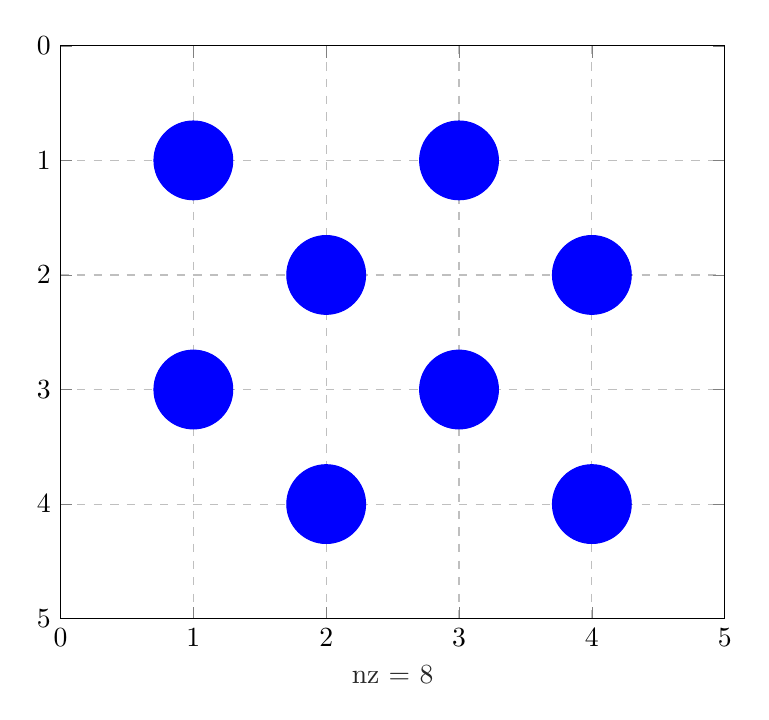
\begin{tikzpicture}

\begin{axis}[%
%width=5.796in,
%height=5.796in,
%at={(2.349in,0.782in)},
scale only axis,
xmin=0,
xmax=5,
xtick={0, 1, 2, 3, 4, 5},
xlabel style={font=\color{white!15!black}},
xlabel={nz = 8},
y dir=reverse,
ymin=0,
ymax=5,
ytick={0, 1, 2, 3, 4, 5},
axis background/.style={fill=white},
xmajorgrids,
ymajorgrids,
grid style={dashed}
]
\addplot [color=blue, draw=none, mark=*, mark options={solid, blue}, mark size = 0.5 cm, forget plot]
  table[row sep=crcr]{%
1	1\\
1	3\\
2	2\\
2	4\\
3	1\\
3	3\\
4	2\\
4	4\\
};
\end{axis}
\end{tikzpicture}%
%%	% This file was created by matlab2tikz.
%
%The latest updates can be retrieved from
%  http://www.mathworks.com/matlabcentral/fileexchange/22022-matlab2tikz-matlab2tikz
%where you can also make suggestions and rate matlab2tikz.
%
\definecolor{mycolor1}{rgb}{0.00000,0.44700,0.74100}%
%
\begin{tikzpicture}

\begin{axis}[%
width=1.99in,
height=1.99in,
at={(1.318in,3.406in)},
scale only axis,
xmin=0,
xmax=9,
xlabel style={font=\color{white!15!black}},
xlabel={nz = 12},
y dir=reverse,
ymin=0,
ymax=9,
axis background/.style={fill=white}
]
\addplot [color=mycolor1, draw=none, mark size=2.3pt, mark=*, mark options={solid, mycolor1}, forget plot]
  table[row sep=crcr]{%
1	1\\
1	2\\
2	2\\
3	3\\
4	3\\
4	4\\
5	5\\
5	6\\
6	6\\
7	7\\
8	7\\
8	8\\
};
\end{axis}

\begin{axis}[%
width=1.99in,
height=1.99in,
at={(4.742in,3.406in)},
scale only axis,
xmin=0,
xmax=9,
xlabel style={font=\color{white!15!black}},
xlabel={nz = 24},
y dir=reverse,
ymin=0,
ymax=9,
axis background/.style={fill=white}
]
\addplot [color=mycolor1, draw=none, mark size=2.3pt, mark=*, mark options={solid, mycolor1}, forget plot]
  table[row sep=crcr]{%
1	1\\
1	3\\
1	5\\
1	7\\
2	2\\
2	4\\
2	6\\
2	8\\
3	1\\
3	3\\
3	5\\
3	7\\
4	2\\
4	4\\
4	6\\
4	8\\
5	5\\
5	7\\
6	6\\
6	8\\
7	5\\
7	7\\
8	6\\
8	8\\
};
\end{axis}

\begin{axis}[%
width=1.99in,
height=1.99in,
at={(1.318in,0.642in)},
scale only axis,
xmin=0,
xmax=9,
xlabel style={font=\color{white!15!black}},
xlabel={nz = 16},
y dir=reverse,
ymin=0,
ymax=9,
axis background/.style={fill=white}
]
\addplot [color=mycolor1, draw=none, mark size=2.3pt, mark=*, mark options={solid, mycolor1}, forget plot]
  table[row sep=crcr]{%
1	5\\
1	7\\
2	6\\
2	8\\
3	5\\
3	7\\
4	6\\
4	8\\
5	5\\
5	7\\
6	6\\
6	8\\
7	5\\
7	7\\
8	6\\
8	8\\
};
\end{axis}

\begin{axis}[%
width=1.99in,
height=1.99in,
at={(4.742in,0.642in)},
scale only axis,
xmin=0,
xmax=9,
xlabel style={font=\color{white!15!black}},
xlabel={nz = 8},
y dir=reverse,
ymin=0,
ymax=9,
axis background/.style={fill=white}
]
\addplot [color=mycolor1, draw=none, mark size=2.3pt, mark=*, mark options={solid, mycolor1}, forget plot]
  table[row sep=crcr]{%
1	1\\
2	2\\
3	3\\
4	4\\
5	5\\
6	6\\
7	7\\
8	8\\
};
\end{axis}
\end{tikzpicture}%
%%	\label{fig:SpyScatter}
%%	\caption{Sparsity Plot-Scattering Block Matrix}
%%\end{figure}
%
%Similarly, for $L^{0,+}  \Sigma_{f,11}^{0} L$ we have
%\begin{equation}
%L^{0,+}  \Sigma_{f,11}^{0} L = 
%		\begin{pmatrix}
%			\frac{1}{2} \chi_{1}\nu\sigma_{f,1,1} & 0 & \chi_{1}\frac{1}{2} \nu\sigma_{f,1,1} & 0 \\
%			0 & \frac{1}{2} \chi_{1}\nu\sigma_{f,1,2} & 0 & \frac{1}{2} \chi_{1}\nu\sigma_{f,1,2}  \\
%			\frac{1}{2} \chi_{1}\nu\sigma_{f,1,1} & 0 & \frac{1}{2} \chi_{1}\nu\sigma_{f,1,1} & 0 \\
%			0 & \frac{1}{2} \chi_{1}\nu\sigma_{f,1,2} & 0 & \frac{1}{2}\chi_{1} \nu\sigma_{f,1,2}
%	\end{pmatrix}.
%\end{equation}
%
%For our model problem, $\mathbf{H_{z}^{-1}} \geq 0$ and has the form \cite{greenbaum1997iterative}
%\begin{equation}
%	\mathbf{H_{z}^{-1}} = \begin{pmatrix}
%  \begin{pmatrix}
%  x & 0 \\
%  x & x
%  \end{pmatrix} & \bigzero & \bigzero & \bigzero \\
%  \bigzero & 
%  \begin{pmatrix}
%  x & x \\
%  0 & x
%  \end{pmatrix} & \bigzero & \bigzero \\
%  \bigzero & \bigzero & \begin{pmatrix}
%  x & 0 \\
%  x & x
%  \end{pmatrix} & \bigzero \\
%  \bigzero & \bigzero & \bigzero & \begin{pmatrix}
%  x & x \\
%  0 & x
%  \end{pmatrix}
%\end{pmatrix},
%\end{equation}
%and $\mathbf{L}^{+}  \mathbf{\Sigma_{f}} \mathbf{L}$ has the form
%\begin{equation}
%\mathbf{L}^{+}  \mathbf{\Sigma_{f}} \mathbf{L} = \frac{1}{2}
%	\begin{pmatrix}
%		\chi_{1} \nu \sigma_{f,1} I_{L} & \chi_{1}\nu \sigma_{f,1} I_{L}& \chi_{1}\nu \sigma_{f,2} I_{L} & \chi_{1} \nu \sigma_{f,2} I_{L} \\
%		\chi_{1}\nu \sigma_{f,1} I_{L} & \chi_{1}\nu \sigma_{f,1} I_{L}& \chi_{1}\nu \sigma_{f,2} I_{L} & \chi_{1}\nu \sigma_{f,2} I_{L} \\
%		\chi_{2}\nu \sigma_{f,1} I_{L} & \chi_{2}\nu \sigma_{f,1} I_{L}& \chi_{2}\nu \sigma_{f,2} I_{L} & \chi_{2}\nu \sigma_{f,2} I_{L} \\
%		\chi_{2}\nu \sigma_{f,1} I_{L} & \chi_{2}\nu \sigma_{f,1} I_{L}& \chi_{2}\nu \sigma_{f,2} I_{L} & \chi_{2}\nu \sigma_{f,2} I_{L}
%	\end{pmatrix}.
%\end{equation}
%Therefore, the matrix $\mathbf{H_{z}^{-1}} \mathbf{L}^{+}  \mathbf{\Sigma_{f}} \mathbf{L}$ has the form
%\begin{equation}
%	\mathbf{H_{z}^{-1}} \mathbf{L}^{+}  \mathbf{\Sigma_{f}} \mathbf{L} = \begin{pmatrix}
%		\LTx & \LTx & \LTx & \LTx \\
%		\UTx & \UTx & \UTx & \UTx \\
%		\LTx & \LTx & \LTx & \LTx \\
%		\UTx & \UTx & \UTx & \UTx
%	\end{pmatrix},
%\end{equation}
%where $x > 0$ represents a positive entry, and where $I_{L}$ is the identity matrix of size $L$. It follows that each block of the matrix $(\mathbf{H_{z}^{-1}}\mathbf{L}^{+}  \mathbf{\Sigma_{f}} \mathbf{L})^{2}$ is
%\begin{equation}
%	\begin{pmatrix}
%		x & 0 \\ x & x
%	\end{pmatrix}
%\begin{pmatrix}
%		x & x \\ 0 & x
%	\end{pmatrix} =
%\begin{pmatrix}
%		x^2 & x^2 \\ x^2 & x^{2}
%	\end{pmatrix} > 0 \text{ because }
%\begin{pmatrix}
%	\chi_{1} \nu\sigma_{f,1} & \chi_{1}\nu\sigma_{f,2} \\ \chi_{2}\nu\sigma_{f,1} & \chi_{2}\nu\sigma_{f,2}
%	\end{pmatrix} > 0
%\end{equation}
%and $\mathbf{H_{z}^{-1}} \geq 0$. Therefore, $\mathbf{H_{z}^{-1}} \mathbf{L}^{+}  \mathbf{\Sigma_{f}} \mathbf{L}$ is primitive and it follows that $\mathbf{A}(\alpha)$ is primitive since $\mathbf{L}^{+}  \mathbf{\Sigma_{s}} \mathbf{L} \geq 0$ for isotropic scattering. For anisotropic scattering, as long as $\mathbf{L}^{+}  \mathbf{\Sigma_{s}} \mathbf{L} \geq 0$, the previous fact remains valid. When the system is subcritical, $\alpha < 0$ and the matrix $\mathbf{A}(\alpha)$ is primitive. For supercritical systems, $\alpha > 0$ and there is an upper limit $\alpha_{\text{max}}$ such that the matrix $\mathbf{A}(\alpha)$ remains primitive. For $k$-effective eigenvalue problems, $k$ is always positive and therefore the matrix $\mathbf{T}(k)$ is primitive.
%%There are other eigenvalue problems useful for various applications \cite{ronen_comparison_1976}, however 

